%   ██████  ████     ████  ████████   ██████         ████  ██████  ██
%  ██░░░░██░██░██   ██░██ ██░░░░░░   ██░░░░██       █░░░ █░█░░░░  ███
% ██    ░░ ░██░░██ ██ ░██░██        ██    ░░       ░    ░█░█████ ░░██
%░██       ░██ ░░███  ░██░█████████░██        █████   ███ ░░░░░ █ ░██
%░██       ░██  ░░█   ░██░░░░░░░░██░██       ░░░░░   ░░░ █     ░█ ░██
%░░██    ██░██   ░    ░██       ░██░░██    ██       █   ░█ █   ░█ ░██
% ░░██████ ░██        ░██ ████████  ░░██████       ░ ████ ░ ████  ████
%  ░░░░░░  ░░         ░░ ░░░░░░░░    ░░░░░░         ░░░░   ░░░░  ░░░░
%     ██      ██                         ██   ██   ██
%    ████    ░██  █████                 ░░   ░██  ░██
%   ██░░██   ░██ ██░░░██  ██████  ██████ ██ ██████░██      ██████████   ██████
%  ██  ░░██  ░██░██  ░██ ██░░░░██░░██░░█░██░░░██░ ░██████ ░░██░░██░░██ ██░░░░
% ██████████ ░██░░██████░██   ░██ ░██ ░ ░██  ░██  ░██░░░██ ░██ ░██ ░██░░█████
%░██░░░░░░██ ░██ ░░░░░██░██   ░██ ░██   ░██  ░██  ░██  ░██ ░██ ░██ ░██ ░░░░░██
%░██     ░██ ███  █████ ░░██████ ░███   ░██  ░░██ ░██  ░██ ███ ░██ ░██ ██████
%░░      ░░ ░░░  ░░░░░   ░░░░░░  ░░░    ░░    ░░  ░░   ░░ ░░░  ░░  ░░ ░░░░░░

% This program is free software: you can redistribute it and/or modify
% it under the terms of the GNU General Public License as published by
% the Free Software Foundation, either version 3 of the License, or
% (at your option) any later version.

% This program is distributed in the hope that it will be useful,
% but WITHOUT ANY WARRANTY; without even the implied warranty of
% MERCHANTABILITY or FITNESS FOR A PARTICULAR PURPOSE.  See the
% GNU General Public License for more details.

% You should have received a copy of the GNU General Public License
% along with this program.  If not, see <http://www.gnu.org/licenses/>.
\documentclass[english, 10pt]{article}

\usepackage{notes}
\usepackage{inconsolata}
\usepackage[shellescape]{gmp}
\allowdisplaybreaks%
\newcommand{\thiscoursecode}{CMSC 351}
\newcommand{\thiscoursename}{Algorithms}
\newcommand{\thisprof}{Dr.\ Clyde Kruskal}
\newcommand{\me}{Alex Reustle}
\newcommand{\thisterm}{Fall 2017}
\newcommand{\website}{http://cs.umd.edu/class/fall2017/cmsc351/}%chktex 8
\usepackage{ifpdf}
\ifpdf%
\DeclareGraphicsRule{*}{mps}{*}{}
\fi
% \listfiles
% \VerbEnvir{align tikzpicture algorithm}
%%%Headers
\chead{351-Algorithms}
\lhead{\thisterm}

%%%%% TITLE %%%%%
\graphicspath{{../}}
\newcommand{\notefront}{%
\pagenumbering{arabic}
\begin{center}
{\small}
\textbf{\Huge{\noun{\thiscoursecode}}}
{\Huge \par}
{\Large{\noun{\thiscoursename}}}\\
\vspace{0.1in}
\vspace{0in}
\includegraphics[scale=0.3]{umd_cs.jpg} \\
\vspace{0.1in}{\noun\me} \\
{\noun\thisprof} \ $\bullet$ \ {\noun\thisterm} \ $\bullet$ \ {\noun{University of Maryland}} \\
{\ttfamily \url{\website}} \\
\end{center}
}

 \tikzstyle{class}=[
    rectangle,
    draw=black,
    text centered,
    anchor=north,
    text=black,
    text width=2cm,
    shading=axis,
    bottom color={rgb:red,222;green,222;blue,222},
    top color=white,shading angle=45]



%  ██████                   ██
% ░█░░░░██           █████ ░░
% ░█   ░██   █████  ██░░░██ ██ ███████
% ░██████   ██░░░██░██  ░██░██░░██░░░██
% ░█░░░░ ██░███████░░██████░██ ░██  ░██
% ░█    ░██░██░░░░  ░░░░░██░██ ░██  ░██
% ░███████ ░░██████  █████ ░██ ███  ░██
% ░░░░░░░   ░░░░░░  ░░░░░  ░░ ░░░   ░░
\begin{document}
% \renewcommand\familydefault{\sfdefault}
% \sffamily
  % Notes front
  \notefront%
  % Table of Contents and List of Figures
  \tocandfigures%


\section{Maximum Subarray Problem}
Given a sequence of integers, find the largest collection which is a sum of adjacent values. Sequence is in an array with indices from 1 to n.
\[
    3~-5~\underbrace{4~3~-6~4~8}_{Sum = 13}~-5~3~-7~2~1 \\
\]

\subsection{Brute Force solution}
Brute force solution: try every possible sum. (I'd guess it's $n^3$) Sum variable M set to zero. We will allow empty sums (no elements, sum = 0).

% \begin{wrapfigure}{R}{0.3\textwidth}
%     \centering
\begin{algorithm}[H]
$M\gets0$\;
\For{i=1 to n}{\
    \For{j=i to n}{\
        $S\gets0$\;
        \For{k=i to j}{\
            $S = S + A[k]$\;
            $M = \max(M,S)$\;
        }
    }
    \caption{Matrix Subarray Brute Force}
}
\end{algorithm}
% \end{wrapfigure}

Insight: Loops in programs are like summation in Mathematics.%
(for i=1) to n == $\sum_{i=1}^{n}$

Nested loops are nested summations.
$\sum_{i=1}^{n} \sum_{j=i}^{n} \sum_{k=i}^{j} 1$

Simplify summation using summation algebra from the inside out.
$\sum_{i=1}^{n} \sum_{j=i}^{n} j-i+1 $

Tangent: since j is the variable, i and 1 are constants. So it can be separated into two sums.

\subsection{Analysis of the Algorithm}
Actual progress: Change a variable to manage sum. Like integrals in calculus. Every technique in calculus for integrations are matched by similar techniques in summations.
Change of variable by example. See appendix for examples of summation properties.
\begin{align*}
    \sum_{i=1}^{n} \sum_{j=i}^{n} \sum_{k=i}^{j} 1 &= \sum_{i=1}^{n} \sum_{j=i}^{n} j-i+1 & \text{By adding 1 $j-i$ times, and fenceposting} \\
    &= \sum_{i=1}^{n} \sum_{j=1}^{n-i+1} j & \text{By change of variable Method} \\
    &= \s{i=1}{n} \f{(n-i+1)(n-i+2)}{2} & \text{Gausses sum} \\
    &= \f{1}{2}\times \s{i=1}{n} (n-i+1)(n-i+2) & \text{Expanding is error prone. Change variable instead} \\
    &= \f{1}{2}\times \s{n-i+1=1}{n} i(i+1) & \text{substitute i=n-i+1} \\
    &= \f{1}{2}\times \s{i=1}{n} i(i+1) & \text{simplify bounds} \\
    &= \f{1}{2}\times \frac{n(n+1)(n+2)}{3} & \text{magic.} \\
    &= \frac{n(n+1)(n+2)}{6} \\
\end{align*}

This first method is $\Theta{\left(n^3\right)}$.

\subsection{Methods to improve integer list summation algorithm.}
Remember previous sums, do not recalculate known data.

% \begin{wrapfigure}{L}{0.3\textwidth}
\begin{algorithm}[H]
$M\gets0$\;
\For{i=1 to n}{\
    $S\gets0$\;
    \For{j = i to n}{\
        $S = S+A[j]$\;
        $M = \max(M,S)$\
    }
}
\caption{$n^2$ Subarray }
\end{algorithm}
% \end{wrapfigure}
$$
    \sum_{i=1}^{n} \sum_{j=i}^{n} 1 = \sum_{i=1}^n n-i+1 \\
    = \sum_{i=1}^{n} i = \frac{n(n+1)}{2}
$$
This new method is $\Theta{\left(n^2\right)} $.

% Further improvements.
Loosely speaking the maximum sum is just the previous maximum sum, plus the current value.
% $$
%     S[i] = S[i-1]+A[i] \\
%     \max( S[i-1]+A[i], 0)
% $$

% \begin{wrapfigure}{R}{0.3\textwidth}
\begin{algorithm}[H]
$M \gets 0,S \gets 0$\;
\For{i = 1 to n}{\
    $S \gets \max(S+A[i], 0)$\;
    $M = \max(M,S)$\;
}
\caption{Linear Subarray }
\end{algorithm}
% \end{wrapfigure}
The third method is $\Theta{\left(n\right)} $.\newline
Correctness of the algorithm stems from proof by induction on $S = \max(S+A[i], 0)$. This is the Loop Invariant.

$$
\sum_{i=1}^n 1 = n \\
% \Theta{(n)}
$$

\section{Timing analysis}
\textbf{Lower Bound}

No algorithm is Faster than this boundary condition, the lower bound time.

Best Case scenario, very hard to prove in the general case.

\textbf{Upper Bound}

Some Algorithm can obtain upper bound time.

Worst case Scenario.

\subsection{Classes of algorithms}
\subsubsection{$\Theta(n^2)$}
    Bubble sort \\
    Insertion Sort \\
    Selection Sort \\
\subsubsection{$\Theta(n\log(n))$}
    Merge Sort \\
    Heap Sort \\
    Quick Sort \\
\subsubsection{Others}
    Radix Sort

%% ██████           ██      ██       ██            ████████                   ██
% ░█░░░░██         ░██     ░██      ░██           ██░░░░░░                   ░██
% ░█   ░██  ██   ██░██     ░██      ░██  █████   ░██         ██████  ██████ ██████
% ░██████  ░██  ░██░██████ ░██████  ░██ ██░░░██  ░█████████ ██░░░░██░░██░░█░░░██░
% ░█░░░░ ██░██  ░██░██░░░██░██░░░██ ░██░███████  ░░░░░░░░██░██   ░██ ░██ ░   ░██
% ░█    ░██░██  ░██░██  ░██░██  ░██ ░██░██░░░░          ░██░██   ░██ ░██     ░██
% ░███████ ░░██████░██████ ░██████  ███░░██████   ████████ ░░██████ ░███     ░░██
% ░░░░░░░   ░░░░░░ ░░░░░   ░░░░░   ░░░  ░░░░░░   ░░░░░░░░   ░░░░░░  ░░░       ░░

\section{Bubble Sort Analysis}
\begin{algorithm}
\For{i = n downto 2}{%
    \For{j = 1 to i-1}{%
        \If{$A[j] > A[j+1]$}{%
        swap (A[j],A[j+1])\;
        }
    }
    \caption{Bubble Sort}
}
\end{algorithm}

Major Growth Elements of Bubble sort will be Comparisons and Exchanges (swaps).\\

Best case number of comparisons require you to view every element unconditionally. \\
\begin{align*}
    \sum_{i=2}^n \sum_{j=1}^{i-1} 1 &= \sum_{i=2}^{n} i-1 \\
    &= \sum_{i=1}^{n-1} (i+1) -1 \\
    &= \sum_{i=1}^{n-1} i \\
    &= \f{(n-1)n}{2} = \binom{n}{2}& \text{Equivalent to n choose 2}
\end{align*}
Comparisons will always occur, regardless of state of list. \\

Best Case Exchanges occur when the list is sorted. Zero exchanges. \\
Worst Case Exchanges occur when the list is reverse sorted. Same number of exchanges as comparisons. \\

\defn[Random] Each permutation (ordering) of the list is equally likely.

    Rotations of list permutations are equally likely to be in any position, but are not random because they ignore other possible permutations.\\

\subsection{Average Case Analysis}
Count Transpositions. Two elements that are out of order related to each other. See appendix for details about transpositions. \\

In the best case there are no transpositions. \\
In the worst case there are n choose 2 transpositions. Every element is out of order with the number of elements below it.
So the number of transpositions is the number of unique pairs. Which is n choose 2 pairs. \\
In a randomized sample the permutations are equally likely to be out of order greater or lesser,
so the number of average case exchanges will be half the number of comparisons. $\f{n(n-1)}{4}$.


 % ██                                   ██   ██                      ████████                   ██
% ░██                                  ░██  ░░                      ██░░░░░░                   ░██
% ░██ ███████   ██████  █████  ██████ ██████ ██  ██████  ███████   ░██         ██████  ██████ ██████
% ░██░░██░░░██ ██░░░░  ██░░░██░░██░░█░░░██░ ░██ ██░░░░██░░██░░░██  ░█████████ ██░░░░██░░██░░█░░░██░
% ░██ ░██  ░██░░█████ ░███████ ░██ ░   ░██  ░██░██   ░██ ░██  ░██  ░░░░░░░░██░██   ░██ ░██ ░   ░██
% ░██ ░██  ░██ ░░░░░██░██░░░░  ░██     ░██  ░██░██   ░██ ░██  ░██         ░██░██   ░██ ░██     ░██
% ░██ ███  ░██ ██████ ░░██████░███     ░░██ ░██░░██████  ███  ░██   ████████ ░░██████ ░███     ░░██
% ░░ ░░░   ░░ ░░░░░░   ░░░░░░ ░░░       ░░  ░░  ░░░░░░  ░░░   ░░   ░░░░░░░░   ░░░░░░  ░░░       ░░
\section{Insertion Sort with Sentinel}

Every 0 to [i-1] index during the loop will be sorted. \\
ith term is stored in tmp. Values in the sorted subarray which are larger than the tmp value are brought forward individually until tmp > A[j]. A sentinel $-\infty$ is used at $A[0]$, so values don't drop off array. \\

\begin{algorithm}
$A[0] \gets -\infty$\; 
\For{i = 2 to n}{%
    $t \gets A[i]$\;
    $j \gets i-1$\;
    \While{$A[j] \ge t$}{%
        $A[j+1] \gets A[j]$\;
        $j \gets j-1$\;
    }
    $A[j+1] \gets t$\;
}
\caption{Insertion Sort with Sentinel}
\end{algorithm}

\subsection{Analysing Number of Comparisons}

\subsubsection{Best Case Comparisons}
In the case where the array is already correctly sorted, there will be only 1 comparison for each iteration of the other for loop.
It will always evaluate false.
So the number of best case comparisons is just the number of for loop iterations.
\begin{align*}
    \s{i=2}{n} 1 &= (n-2)+1 & \text{Already sorted} \\
    &= n-1
\end{align*}

\subsubsection{Worst Case Comparisons}
In the worst case the array is reverse sorted, and every element must be moved.
The while loop always decrements j to zero to compare against the sentinel value.
\begin{align*}
    \sum_{i=2}^n i &= \left(\sum_{i=1}^{n}i \right)-1 & \text{Reverse Sorted} \\
    &= \f{n(n+1)}{2} -1 & \text{must remove i=1} \\
    &= \f{(n+2)(n-1)}{2}
\end{align*}

\subsubsection{Average Case Comparisons}
In the average case we must determine the probability that a given element will move.
So for evaluation we want the expected value over the set $\sum_{x \in X} P(x)\cdot V(x) $.

Starting at location i, go until reach location j-1.
Probability (P) that 1 element (A[i]) will end up in any location in the subarray is $\f{1}{i}$. Value (V) is number of moves which is (i-j+1).

\begin{align*}
    \s{i=2}{n} \s{j=1}{i} \frac{1}{i} \cdot (i-j+1) &= \s{i=2}{n} \frac{1}{i} \s{j=1}{i} (i-j+1)  &  \text{Pull out 1/i} \\
 &= \s{i=2}{n}\frac{1}{i}\s{j=1}{i} j \\
 &= \s{i=2}{n}\frac{1}{i}\cdot\frac{i(i+1)}{2} \\
 &= \s{i=2}{n}\frac{(i+1)}{2} \\
 &= \frac{1}{2}\left[ \s{i=2}{n}i+1\right] \\
 &= \frac{1}{2}\left[ \s{i=2}{n}i+ \s{i=2}{n}1\right] \\
 &= \frac{1}{2}\left[ \s{i=1}{n}i -1 + (n-1) \right] \\
 &= \frac{1}{2}\left[ \f{(n)(n+1)}{2} -1 + \frac{2(n-1)}{2} \right] \\
 &= \frac{1}{2}\left[ \f{(n^2+n-2)}{2} + \frac{2n-2}{2} \right] \\
 &= \f{(n^2+3n-4)}{4}  \\
 &= \f{(n+4) (n-1)}{4}
\end{align*}


\subsection{Analyzing Exchanges}

\subsubsection{Best Case Exchanges}

Best case number of moves = $2n-1$. There is 1 move in in the $-\infty$
assignment at the top, then in the for loop there are 2 moves per iteration,
moving A[i] into t, and moving it back into the same spot. $1 + 2(n-1) = 2n
-1$.

\subsubsection{Worst Case Exchanges}

Worst case number of moves is 2 for each iteration of outer loop plus worst
case number of comparisons, minus the time when the comparison is false at the
end, of the inner loop, plus 1 for the top assignment. $2(n-1) + COMP - (n-1)
+1 $.

Note the short cut, at each iteration we're doing one more move than
comparison. So just easily take the value already derived for Worst case
comparisons, and add the number of loop iterations, plus 1 for the sentinel
assignment.  $$\frac{(n+2)(n-1)}{2} +n $$

\subsubsection{Average Case Exchanges}

In the average case, whenever there's a comparison, there will always be a
move, except the 1 time per iteration it evaluates false.  So the analysis
method is the same as for the worse case. Since we know the number.  $$\f{(n+4)
(n-1)}{4} + n$$

\begin{rem}

An important trick is to recognize that the moves are related to the
comparisons 1 to 1 and that there will be 1 time when the comparison evaluates
false each iteration, so you subtract that from the final analysis.

\end{rem}


%  ██                                   ██   ██                      ████████                   ██                      ██
% ░██                                  ░██  ░░                      ██░░░░░░                   ░██                     ██
% ░██ ███████   ██████  █████  ██████ ██████ ██  ██████  ███████   ░██         ██████  ██████ ██████   ███     ██     ██    ██████
% ░██░░██░░░██ ██░░░░  ██░░░██░░██░░█░░░██░ ░██ ██░░░░██░░██░░░██  ░█████████ ██░░░░██░░██░░█░░░██░   ░░██  █ ░██    ██    ██░░░░██
% ░██ ░██  ░██░░█████ ░███████ ░██ ░   ░██  ░██░██   ░██ ░██  ░██  ░░░░░░░░██░██   ░██ ░██ ░   ░██     ░██ ███░██   ██    ░██   ░██
% ░██ ░██  ░██ ░░░░░██░██░░░░  ░██     ░██  ░██░██   ░██ ░██  ░██         ░██░██   ░██ ░██     ░██     ░████░████  ██     ░██   ░██
% ░██ ███  ░██ ██████ ░░██████░███     ░░██ ░██░░██████  ███  ░██   ████████ ░░██████ ░███     ░░██    ███░ ░░░██ ██      ░░██████
% ░░ ░░░   ░░ ░░░░░░   ░░░░░░ ░░░       ░░  ░░  ░░░░░░  ░░░   ░░   ░░░░░░░░   ░░░░░░  ░░░       ░░    ░░░    ░░░ ░░        ░░░░░░
%   ████████                    ██   ██                   ██
%  ██░░░░░░                    ░██  ░░                   ░██
% ░██         █████  ███████  ██████ ██ ███████   █████  ░██
% ░█████████ ██░░░██░░██░░░██░░░██░ ░██░░██░░░██ ██░░░██ ░██
% ░░░░░░░░██░███████ ░██  ░██  ░██  ░██ ░██  ░██░███████ ░██
%        ░██░██░░░░  ░██  ░██  ░██  ░██ ░██  ░██░██░░░░  ░██
%  ████████ ░░██████ ███  ░██  ░░██ ░██ ███  ░██░░██████ ███
% ░░░░░░░░   ░░░░░░ ░░░   ░░    ░░  ░░ ░░░   ░░  ░░░░░░ ░░░

\section{Insertion Sort without Sentinel}

Add another comparison in the algorithm so the A[0] term is unnecessary, by checking that you haven't gone past i=1.

\begin{algorithm}[H]
    \For{i=2 to n}{%
        $t\gets A[i]$\;
        $j \gets i-1$\;
        \While{$j > 0 \wedge A[j] > t$}{%
            $A[j+1]\gets A[j]$\;
            $j \gets j-1$\;
        }
        $A[j+1]\gets t$\;
    }
\caption{Insertion Sort w/o Sentinel}
\end{algorithm}

A note about comparisons. We don't count index value comparisons, because index values can easily be stored in registers and won't have the same
cost to check as array value comparisons.

\subsection{Best Case Comparisons}
In the best case, the array is already sorted, so there will just be 1 comparison per iteration of the outer loop. $\s{i=2}{n} 1 = (n-2) + 1 = n-1$

\subsection{Worst Case Comparisons}
In the worst case, the array is reverse sorted, and every ith iteration of the loop must compare against all previous $(i-1)$  elements.
\begin{align*}
    \s{i=2}{n}\s{j=1}{i-1}1 &= \s{i=2}{n} (i-1) \\
    &= \s{i=2}{n} i - \s{i=2}{n} 1 \\
    &= \f{n(n+1)}{2} -1 -(n-1) \\
    &= \f{n(n+1)}{2} -n \\
    &= \f{n^2 + n}{2} -\frac{2n}{2} \\
    &= \f{n^2 - n}{2} \\
    &= \f{n(n-1)}{2} \\
\end{align*}
% $$\frac{n(n-1)}{2}$$


\subsection{Average Case Comparisons}
\begin{rem}
HARMONIC SERIES and brick problem.
How far out can you stack bricks on top of one another? Arbitrarily far out (but not infinitely far out)
$$H_n = \s{i=1}{n}\frac{1}{i} = 1+\frac{1}{2}+\frac{1}{3}+\frac{1}{4}+\frac{1}{5}+\cdots \approx \ln{n}+1$$
$$H_n -1 = \s{i=2}{n}\frac{1}{i} = \frac{1}{2}+\frac{1}{3}+\frac{1}{4}+\frac{1}{5}+\cdots \approx \ln{n}$$
Harmonic Series come up again and again because of the idea that something has a $\frac{1}{i}$ chance of happening in an iteration.
\end{rem}
What are we saving when we don't have a sentinel? In the event that the ith element is the smallest element in the A[1..i-1] sub-array, we will descend all
the way to the 1st index of the list. If that happens, we won't have the 1 extra step of comparing against the sentinel. So only when the ith element is
the smallest seen thus far do we save 1 step.
Probability that current ith element is smallest in sub array is $\frac{1}{i}$. The value when that occurs is 1.
Thus over all n elements of the array, on average the sentinel would have cost us $\s{i=2}{n}\frac{1}{i} = H_n -1$ comparisons.

So average case comparisons without sentinel is average case with sentinel minus average cost of sentinel.
$\frac{(n-1)(n+4)}{4}-(H_n -1) \approx \frac{(n-1)(n+4)}{4}-\ln{n}$.

\subsection{Exchanges}
Removing the sentinel from insertion sort adds no new exchanges, nor does it alter when a change might have been done already.
Therefore, the best, worst and average cases are all the same as insertion sort with sentinel.


%   ████████          ██                   ██   ██                      ████████                   ██
%  ██░░░░░░          ░██                  ░██  ░░                      ██░░░░░░                   ░██
% ░██         █████  ░██  █████   █████  ██████ ██  ██████  ███████   ░██         ██████  ██████ ██████
% ░█████████ ██░░░██ ░██ ██░░░██ ██░░░██░░░██░ ░██ ██░░░░██░░██░░░██  ░█████████ ██░░░░██░░██░░█░░░██░
% ░░░░░░░░██░███████ ░██░███████░██  ░░   ░██  ░██░██   ░██ ░██  ░██  ░░░░░░░░██░██   ░██ ░██ ░   ░██
%        ░██░██░░░░  ░██░██░░░░ ░██   ██  ░██  ░██░██   ░██ ░██  ░██         ░██░██   ░██ ░██     ░██
%  ████████ ░░██████ ███░░██████░░█████   ░░██ ░██░░██████  ███  ░██   ████████ ░░██████ ░███     ░░██
% ░░░░░░░░   ░░░░░░ ░░░  ░░░░░░  ░░░░░     ░░  ░░  ░░░░░░  ░░░   ░░   ░░░░░░░░   ░░░░░░  ░░░       ░░

\section{Selection Sort}
Summary: Find biggest element, put at bottom of list, recurse for sub array.

\begin{algorithm}[H]
    \For{i=n downto 2}{%
        $k\gets 1$\;
        \For{j=2 to i}{%
            \If{$A[j] > A[k]$}{%
                $k \gets j$\;
            }
        }
        swap (A[k], A[i])\;
    }
    \caption{Selection Sort}
\end{algorithm}

\subsection{Comparisons}
The comparison is always run, so the comparison value should be the same for all cases.
\begin{align*}
    \s{i=2}{n}\s{j=2}{i}1 &= \s{i=2}{n} (i-1) \\
    & = \frac{(n-1)n}{2}\\
\end{align*}

\subsection{Exchanges}
Exchanges don't occur inside the conditional, so exchanges number is simply n-1.

How many times do we exchange a number with itself? How many times does i=k?
$\sum 1/i = H_n$



 % ████     ████                                   ████████                   ██
% ░██░██   ██░██                 █████            ██░░░░░░                   ░██
% ░██░░██ ██ ░██  █████  ██████ ██░░░██  █████   ░██         ██████  ██████ ██████
% ░██ ░░███  ░██ ██░░░██░░██░░█░██  ░██ ██░░░██  ░█████████ ██░░░░██░░██░░█░░░██░
% ░██  ░░█   ░██░███████ ░██ ░ ░░██████░███████  ░░░░░░░░██░██   ░██ ░██ ░   ░██
% ░██   ░    ░██░██░░░░  ░██    ░░░░░██░██░░░░          ░██░██   ░██ ░██     ░██
% ░██        ░██░░██████░███     █████ ░░██████   ████████ ░░██████ ░███     ░░██
% ░░         ░░  ░░░░░░ ░░░     ░░░░░   ░░░░░░   ░░░░░░░░   ░░░░░░  ░░░       ░░
\section{Merge Sort}
Divide and Conquer. Recursively split array in half down to 1 element, then merge sorted sublists.
First call of Mergesort is (A,1,n) \\


\begin{algorithm}[H]
    MERGESORT (A,p,r)\;
    //p and r are indices in array defining sub array.\;
    \If{p<r}{%
        $q \gets \lfloor{\frac{p+r}{2}}\rfloor$\;
        MERGESORT (A,p,q)\;
        MERGESORT (A,q+1,r)\;
        MERGE (A, (p,q), (q+1,r))\;
    \caption{Merge Sort}
    }
\end{algorithm}


\subsection{Merge Comparison analysis}
\subsubsection{Equal length arrays}
Merge algorithm is linear over 2 sorted lists of same size (n). Total number of comparisons in the worst case during merge is $2n-1$, best case comparisons is n, where
1 array is strictly greater than the other.

Can't do better than $2n-1$ in worst case, because worst case situation is 2 lists with interleaved values. In this case the granularity of difference is on the scale of 1 value. So you must check every value to ensure against that. The last remaining value of 2 lists is not compared, which leads to 2n-1.

This gives us very tight bounds and lets us know everything there is to know about merging.

\subsubsection{Different length arrays}
Arrays of size m and n where $m\le n$ Worst case comparisons = $m+n-1$

When $m<<n$ you can get close to $\log n$ running time using binary search. But when m is close to n you are much closer to the $m+n-1$ worst case.


\subsection{Mergesort Comparison Analysis}
\textbf{Exact Number of Comparisons During a merge}
$$ (q-p+1) + (r-(q+1)+1) -1 = (r-p)\; \text{comparisons} $$
starting at index p and ending at index q. So for the full list, where p=1 and q=n a MERGESORT will start with (n-1) comparisons and have the following behavior.

\begin{tikzpicture}[level/.style={sibling distance=55mm/#1, level distance = 1.5cm}]
\node  (z){$n-1$}
    child {node  (1a) {$\frac{n}{2}-1$}
        child {node  (2a) {$\frac{n}{2^2}-1$}
            child {node {$\vdots$}
                child {node  (3a) {$\left(\frac{n}{2^k}-1\right)$}
                    child {node  (01) {0}}
                    child {node  (02) {0}}
                }
                child {node  (3b) {$\left(\frac{n}{2^k}-1\right)$}
                    child {node  (03) {0}}
                    child {node  (04) {0}}
                }
            }
            child {node {$\vdots$}}
        }
        child {node  (2b) {$\frac{n}{2^2}-1$}
            child {node {$\vdots$}}
            child {node {$\vdots$}}
        }
    }
    child {node  (1b) {$\frac{n}{2}-1$}
        child {node  (2c) {$\frac{n}{2^2}-1$}
            child {node {$\vdots$}}
            child {node {$\vdots$}}
        }
        child {node  (2d) {$\frac{n}{2^2}-1$}
            child {node {$\vdots$}}
            child {node {$\vdots$}
                child {node  (3c) {$\left(\frac{n}{2^k}-1\right)$}}
                child {node  (3d) {$\left(\frac{n}{2^k}-1\right)$}
                    child{node (05) {0}}
                    child{node (06) {0}
                        child [grow=right] {node (eq0) {$=$} edge from parent[draw=none]
                            child [grow=right] {node (eq0) {$0n$} edge from parent[draw=none]
                                child [grow=up] {node (eq1) {$2^k \left( \frac{n}{2^k}-1 \right)$} edge from parent[draw=none]
                                      child [grow=up] {node (eq2) {$\vdots$} edge from parent[draw=none]
                                          child [grow=up] {node (eq3) {$2^2 \left( \frac{n}{2^2}-1 \right)$} edge from parent[draw=none]
                                              child [grow=up] {node (eq4) {$2^1\left( \frac{n}{2}-1 \right)$} edge from parent[draw=none]
                                                  child [grow=up] {node (eq5) {$2^0\left(n-1 \right)$} edge from parent[draw=none]}
                                      }
                                    }
                                  }
                                }
                            child [grow=down] {node (eq6) {$\s{i=0}{\lg n} 2^i (\frac{n}{2^i}-1)$}edge from parent[draw=none]}
                            }
                        }
                    }
                }
            }
        }
};
\path (1a) -- (1b) node [midway] {+};
\path (2a) -- (2b) node [midway] {+};
\path (2b) -- (2c) node [midway] {+};
\path (2c) -- (2d) node [midway] {+};
\path (3a) -- (3b) node [midway] {+};
\path (3c) -- (3b) node (3cent) [midway] {+};
\path (3c) -- (3cent) node (3cent) [midway] {$\cdots$};
\path (3cent) -- (3a) node (3cent) [midway] {$\cdots$};
\path (3c) -- (3d) node [midway] {+};
\path (01) -- (02) node [midway] {+};
\path (03) -- (04) node [midway] {+};
\path (05) -- (06) node [midway] {+};
\path (01) -- (06) node (0cent) [midway] {+};
\path (0cent) -- (05) node [midway] {$\cdots$};
\path (0cent) -- (02) node [midway] {$\cdots$};
\path (eq0) -- (eq1) node [midway] {+};
\path (eq2) -- (eq1) node [midway] {+};
\path (eq2) -- (eq3) node [midway] {+};
\path (eq4) -- (eq3) node [midway] {+};
\path (eq5) -- (eq4) node [midway] {+};
\path (eq0) -- (eq6) node [midway] {=};
\end{tikzpicture}


Because this gives $\lg n$ terms, we can make it a little easier by dropping the bottom row, which sums to 0 anyway, because it's $0n$.
\begin{align*}
    \s{i=0}{\lg n-1} 2^i (\frac{n}{2^i}-1) &= \s{i=0}{\lg n-1} (n-2^i) \\
    &= \s{i=0}{\lg n-1} n - \s{i=0}{\lg n-1} 2^i \\
    &= (n\lg n) - (2^{\lg n-1 +1} -1) & \text{geometric series} \\
    &= (n\lg n ) - (n-1) \\
    &= n\lg n  - n+1 \\
\end{align*}
\subsection{Merge Sort Recurrence}
When expressed as a recurrence relation, the mergesort algorithm given previously behaves like 
\begin{align*}
    S(n) &= S\left( \frac{n}{2} \right)+S\left( \frac{n}{2} \right)+n-1 \\
    &= 2\cdot S\left( \frac{n}{2} \right)+n-1 \\
    \intertext{Which gives the following recurrence relation} 
    S(0) &= S(1) = 0 & \text{Base case of 0 comparisons with 0 or 1 element}\\
    S(n) &= S\left(\lfloor \frac{n}{2}\rfloor \right) + S\left( \lceil \frac{n}{2} \rceil \right)
\end{align*}

 % ██            ██                                        ██            ██   ██   ██                            ██   ██
% ░██           ░██            █████                      ████          ░░   ░██  ░██                           ░██  ░░
% ░██ ███████  ██████  █████  ██░░░██  █████  ██████     ██░░██   ██████ ██ ██████░██      ██████████   █████  ██████ ██  █████
% ░██░░██░░░██░░░██░  ██░░░██░██  ░██ ██░░░██░░██░░█    ██  ░░██ ░░██░░█░██░░░██░ ░██████ ░░██░░██░░██ ██░░░██░░░██░ ░██ ██░░░██
% ░██ ░██  ░██  ░██  ░███████░░██████░███████ ░██ ░    ██████████ ░██ ░ ░██  ░██  ░██░░░██ ░██ ░██ ░██░███████  ░██  ░██░██  ░░
% ░██ ░██  ░██  ░██  ░██░░░░  ░░░░░██░██░░░░  ░██     ░██░░░░░░██ ░██   ░██  ░██  ░██  ░██ ░██ ░██ ░██░██░░░░   ░██  ░██░██   ██
% ░██ ███  ░██  ░░██ ░░██████  █████ ░░██████░███     ░██     ░██░███   ░██  ░░██ ░██  ░██ ███ ░██ ░██░░██████  ░░██ ░██░░█████
% ░░ ░░░   ░░    ░░   ░░░░░░  ░░░░░   ░░░░░░ ░░░      ░░      ░░ ░░░    ░░    ░░  ░░   ░░ ░░░  ░░  ░░  ░░░░░░    ░░  ░░  ░░░░░

\section{Integer Arithmetic}
\subsection{Addition}
Just like in elementary addition, the time to add 2 n digit numbers is proportional to the number of digits. $\Theta(n)$.
Since each digit must be used to compute the sum this is the right order for best case time.

\begin{center}
\opadd{1234}{5678}\qquad
\end{center}

We assume that each digital addition takes constant time (with carry also, so ignore that little trouble spot) and label this constant $\alpha$. The time to add 2 n digit numbers is then $\alpha(n)$.

\subsection{Problem size}

If we were attempting to determine if a number was prime we would divide it by consecutive primes up to the square root of that number.
In Computer Science we want to approach all problems in terms of the problem size. So we should look at both in terms of the NUMBER OF DIGITS,
and not the size of the number. So while the prime identification problem is $\Theta{\sqrt{N}}$ where N is the number,
expressed in binary as $2^n$, n being the number of binary digits. $\Theta(2^{\frac{n}{2}})$. Giving an exponential time algorithm.

\subsection{Multiplication}

Elementary school approach to multiplication runs in $n^2$ time because every digit on top is multiplied by every digit on the bottom. There are $2n(n-1)$ atomic additions in this elementary approach as described in class.\\
\begin{center}
    \opmul[displayintermediary=all]{1234}{5678}
\end{center}

\subsubsection{Recursive Multiplication}

By memorizing the numbers in large bases, say base 100, 2 digit decimal numbers can be treated as 1 digit numbers in base 100.
That makes the multiplication easier, because there are fewer steps.

To generalize this for n digit numbers, treat them as base $10^{\frac{n}{2}}$ and cut each in half. Each has $\frac{n}{2}$ digits, and we know the base.
Then, recurse through this method until we reach a base we really have memorized the table for. Then multiply them as 2 2 digit numbers, and pull out the answer.


% cd x ab equation.
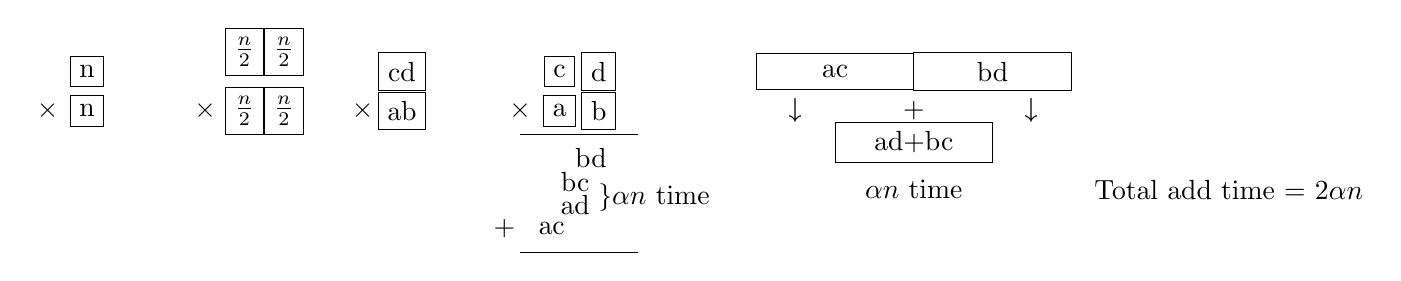
\begin{tikzpicture}
    \node[draw] at (0.5,0) {n};
    \node at (0,0) {$\times$};
    \node[draw] at (0.5,0.5) {n};

    \node[draw] at (2.5,0) {$\frac{n}{2}$};
    \node[draw] at (3,0) {$\frac{n}{2}$};
    \node at (2,0) {$\times$};
    \node[draw] at (2.5,0.75) {$\frac{n}{2}$};
    \node[draw] at (3,0.75) {$\frac{n}{2}$};

    \node[draw] at (4.5,0) {ab};
    \node at (4,0) {$\times$};
    \node[draw] at (4.5,0.5) {cd};

    \node[draw] at (6.5,0) {a};
    \node[draw] at (7,0) {b};
    \node at (6,0) {$\times$};
    \node[draw] at (6.5,0.5) {c};
    \node[draw] at (7,0.5) {d};
    \draw(6,-0.3) -- (7.5,-0.3);
    \node at (6.9,-0.6) {bd};
    \node at (6.7,-0.9) {bc};
    \node at (6.7,-1.2) {ad};
    \node at (7.7,-1.1) {\textbraceright $\alpha n$ time};
    \node at (6.4,-1.5) {ac};
    \node at (5.8,-1.5) {+};
    \draw(6,-1.8) -- (7.5,-1.8);

    \node[draw,minimum width = 2cm, minimum height = 0.45cm] at (10,0.5) {ac};
    \node[draw,minimum width = 2cm] at (12,0.5) {bd};
    \node at (9.5,0) {\textdownarrow};
    \node at (11,0) {+};
    \node at (12.5,0) {\textdownarrow};
    \node[draw,minimum width = 2cm] at (11,-0.4) {ad+bc};
    % \node at (9.5,-1) {$\frac{n}{2}$};
    % \node at (12.5,-1) {$\frac{n}{2}$};
    \node at (11,-1) {$\alpha n$ time};
    \node at (15,-1) {Total add time = $2\alpha n$};
\end{tikzpicture}

$ac$ is an n digit number, as are $ad$, $bc$, $bd$. When adding, $bd$ is not shifted, but $ad$, and $bc$ are shifted by $\frac{n}{2}$ digits, and $ac$ is shifted by n digits.
Since there's no overlap for $ac$ and $bd$, you can add them simply by concatenation.
$ad + bc$ takes $\alpha n$ time. That value plus the center (overlapping) segment of $ac+bd$ is also $\alpha n$.
\newline
\newline
So without writing out the algorithm: $M(n) = 4M\left( \frac{n}{2} \right)+2\alpha n$ which gives us a nice recursion to work on. Let's assume the time to multiply in the base case is $\mu$. The base case is when both of our numbers are 1 digit long $M(1) = \mu$.

\begin{tikzpicture}
    \Tree [.$2\alpha n$ $\cdots$ $\cdots$ $\cdots$ [.$2\alpha\frac{n}{2}$ $\cdots$ $\cdots$ $\cdots$
        [.$\cdots$ $\cdots$ $\cdots$ $\cdots$ [.$2\alpha\frac{n}{2^k}$ $\mu$ $\mu$ $\mu$ $\mu$ ]]]]
        \node[draw] at (4,0) {$4^0(2\alpha n)$};
        \node[draw] at (5,-1) {$4^1(2\alpha \frac{n}{2})$};
        \node[draw] at (6,-2) {$\vdots$};
        \node[draw] at (8,-3) {$4^{k}(2\alpha \frac{n}{2^{k}})$};
        \node[draw] at (8,-4) {$4^{{\lg(n)}}\mu$};
\end{tikzpicture}

Which is fun, I'm having fun. 

\begin{align*}
    \text{atomic actions} &= \s{i=0}{\lg(n)-1} (4^i (2\alpha\frac{n}{2^i}) ) + 4^{\lg(n)}\mu \\
    &=2\alpha n \s{i=0}{\lg n-1}\frac{4^i}{2^i} \cdots\\
    &=2\alpha n \s{i=0}{\lg n-1}{2^i} \cdots\\
    &=2\alpha n \left( 2^{\lg n -1 +1} -1 \right) \cdots& & \text{geometric series} \\
    &=2\alpha n \left( n-1 \right) + 4^{\lg(n)}\mu\\
    &=2\alpha n \left( n-1 \right) + n^{\lg(4)}\mu & 4^{\lg(n)} \mu = n^{\lg 4} \mu \\
    &=2\alpha n \left( n-1 \right) + n^{2}\mu & n^{\lg 4} \mu = n^2 \mu \\
    &=2\alpha n \left( n-1 \right)+n^2 \mu
\end{align*}

We're doing $n^2$ multiplications and $n^2$ additions, so our application of
recursion didn't improve the running time of our algorithm. There's a better
way!

\subsection{Better Multiplication}

With the distributive law $(a+b)(c+d) = ac + ad + bc + bd$, we can use this property to improve the fast multiplication algorithm.
This will let us replace 1 recursive multiplication with 1 new addition and 1 subtraction, as we shall see.
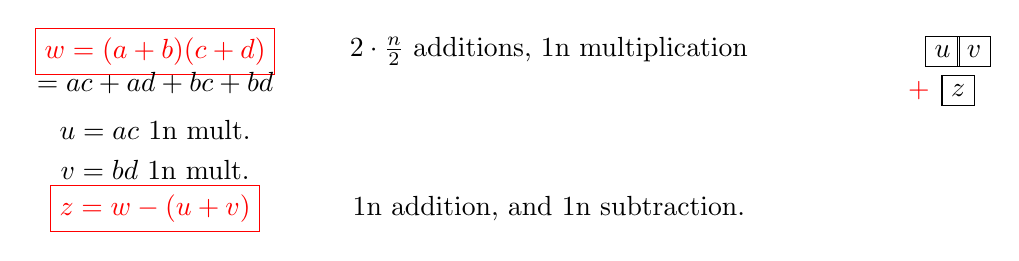
\begin{tikzpicture}
    \node[draw, color=red] at (0,0) {$w=(a+b)(c+d)$};
    \node at (5,0) {$2\cdot\frac{n}{2}$ additions, 1n multiplication};
    \node at (0,-0.4) {$=ac+ad+bc+bd$};
    \node at  (0,-1) {$u=ac$ 1n mult.};
    \node at (0,-1.5) {$v=bd$ 1n mult.};
    \node[draw, color=red] at (0,-2) {$z=w-(u+v)$};
    \node at (5,-2) {1n addition, and 1n subtraction. };
    \node[draw] at (10,0) {$u$};
    \node[draw] at (10.4,0) {$v$};
    \node[draw] at (10.2,-0.5) {$z$};
    \node[color=red] at (9.7,-0.5) {$+$};
\end{tikzpicture}



By the same logic as the earlier multiplication algorithm, $ac$ and $bd$ are
shifted by n bits, and can be concatenated.  Let $w=(a+b)(c+d)$, and $z = w
-(ac + bd) = (ad+bc)$ so to calculate $z$ takes 3 Multiplications, 3 additions
and 1 subtraction. Let's treat the subtraction as an addition, 4 additions.
As such, the recursion for this algorithm is $T(n) = 3T\left( \frac{n}{2} \right)+4\alpha n, T(1) = \mu$.

\begin{align*}
    \s{i=0}{\lg n-1} 3^i \left( 4\alpha \frac{n}{2^i} \right) + 3^{\lg n}\mu &= 4\alpha n \sum \frac{3^i}{2^i} &+n^{\lg 3}\mu \\
    &= 4\alpha n \cdot \frac{{\left(\frac{3}{2} \right)}^{\lg n -1 +1}-1}{\frac{3}{2}-1} &\vdots\\
    &= 4\alpha n \cdot \frac{{\left(\frac{3}{2} \right)}^{\lg n }-1}{\frac{1}{2}}  &\vdots\\
    &= 8\alpha n \left[ n^{\lg \left( \frac{3}{2} \right)}-1 \right]  &\vdots\\
    &= 8\alpha n \left[ n^{\lg 3 - \lg 2}-1 \right]  &\vdots\\
    &= 8\alpha n \left[ \frac{n^{\lg 3}}{n^{\lg 2}}-1 \right]  &\vdots\\
    &= 8\alpha n \left[ \frac{n^{\lg 3}}{n}-1 \right]  &\vdots\\
    &= 8\alpha \left[ {n^{\lg 3}} -n \right] + n^{\lg 3}\mu\\
    &\approx {n^{\lg 3}}\left[ 8\alpha +\mu \right] \\
    &\approx {n^{1.57}}\left[ 8\alpha +\mu \right] \\
\end{align*}

This is $O(n^{1.57})$, a better result than the previous algorithm.


 % ███████                                          ██                     ████     ████                     ██
% ░██░░░░██                                        ░░                     ░██░██   ██░██                    ░██
% ░██   ░██   █████   █████  ██   ██ ██████  ██████ ██  ██████  ███████   ░██░░██ ██ ░██  ██████    ██████ ██████  █████  ██████
% ░███████   ██░░░██ ██░░░██░██  ░██░░██░░█ ██░░░░ ░██ ██░░░░██░░██░░░██  ░██ ░░███  ░██ ░░░░░░██  ██░░░░ ░░░██░  ██░░░██░░██░░█
% ░██░░░██  ░███████░██  ░░ ░██  ░██ ░██ ░ ░░█████ ░██░██   ░██ ░██  ░██  ░██  ░░█   ░██  ███████ ░░█████   ░██  ░███████ ░██ ░
% ░██  ░░██ ░██░░░░ ░██   ██░██  ░██ ░██    ░░░░░██░██░██   ░██ ░██  ░██  ░██   ░    ░██ ██░░░░██  ░░░░░██  ░██  ░██░░░░  ░██
% ░██   ░░██░░██████░░█████ ░░██████░███    ██████ ░██░░██████  ███  ░██  ░██        ░██░░████████ ██████   ░░██ ░░██████░███
% ░░     ░░  ░░░░░░  ░░░░░   ░░░░░░ ░░░    ░░░░░░  ░░  ░░░░░░  ░░░   ░░   ░░         ░░  ░░░░░░░░ ░░░░░░     ░░   ░░░░░░ ░░░
 % ████████                                      ██
% ░██░░░░░                                      ░██
% ░██        ██████  ██████ ██████████  ██   ██ ░██  ██████
% ░███████  ██░░░░██░░██░░█░░██░░██░░██░██  ░██ ░██ ░░░░░░██
% ░██░░░░  ░██   ░██ ░██ ░  ░██ ░██ ░██░██  ░██ ░██  ███████
% ░██      ░██   ░██ ░██    ░██ ░██ ░██░██  ░██ ░██ ██░░░░██
% ░██      ░░██████ ░███    ███ ░██ ░██░░██████ ███░░████████
% ░░        ░░░░░░  ░░░    ░░░  ░░  ░░  ░░░░░░ ░░░  ░░░░░░░░
\section{Recursion Master Formula}
$$ T(n) = aT(\frac{n}{b}) + cn^d, \; T(1)=f$$

Kruskal claims this is a better formula than the master theorem in the book, easier to use and more applicable.
Let's solve using tree method.

\begin{tikzpicture}
    \Tree [.$cn^d$ $\cdots$ $\cdots$ $\cdots$ [.$c\frac{n}{b}^d$ $\cdots$ $\cdots$ $\cdots$
        [.$c\frac{n}{b^2}^d$ $\cdots$ $\cdots$ $\cdots$
            [.$\cdots$ $\cdots$ $\cdots$ $\cdots$ [.$c\frac{n}{b^{n-1}}^d$ $f$ $f$ $f$ $f$ ]]]]]
        \node at (9,1) {num rows};
        \node at (11,1) {sum};
        \node[draw] at (9,0) {$1$};
        \node[draw] at (9,-1) {$a$};
        \node[draw] at (9,-2) {$a^2$};
        \node[draw] at (9,-4) {$a^{n-1}$};
        \node[draw] at (9,-5) {$a^n$};
        \node at (10,-3) {$\vdots$};
        \node[draw] at (11,0) {$cn^d$};
        \node[draw] at (11,-1) {$ac(\frac{n}{b})^d$};
        \node[draw] at (11,-2) {$a^2c(\frac{n}{b^2})^d$};
        \node[draw] at (11,-4) {$a^{n-1}c(\frac{n}{b^{n-1}})^d$};
        \node[draw] at (11,-5) {$fa^{\log_b n}$};
\end{tikzpicture}

You will get $\log_b n$ levels, the branching factor is a.

\begin{align*}
    \s{i=0}{\log_b n-1} a^i c {(\frac{n}{b^i})}^d &= cn^d \s{i=0}{\log_b n-1}\frac{a^i}{{b^i}^d} &+ fn^{\log_b a} \\
    &= cn^d \s{i=0}{\log_b n-1}\frac{a^i}{{b^d}^i} &+ \vdots\\
    &= cn^d \s{i=0}{\log_b n-1}{\left(  \frac{a}{b^d}\right)}^i \\
    &= cn^d \left(\frac{{(\frac{a}{b^d})}^{\log_b n}-1}{\frac{a}{b^d}-1}\right) \\
    &=cn^d \left( \f{n^{\log_b (\frac{a}{b^d})} -1 }{\frac{a}{b^d}-1 } \right) \\
    &=cn^d \left( \f{n^{\log_b {a} -\log_b{b^d}} -1 }{\frac{a}{b^d}-1 } \right) \\
    &=cn^d \left( \f{n^{\log_b {a} -d} -1 }{\frac{a}{b^d}-1 } \right) \\
    &= \f{cn^{\log_b {a}} -cn^d }{\frac{a}{b^d}-1 } +\vdots \\
    &=\frac{cn^{\log_b a}}{\frac{a}{b^d}-1} - \frac{cn^d}{\frac{a}{b^d}-1} + fn^{\log_b a} \\
    &=\left( \frac{c}{\frac{a}{b^d}-1}+f \right)\cdot{n^{\log_b a}} - \frac{cn^d}{\frac{a}{b^d}-1} \\
\end{align*}

This formula can't apply to the situation when the value of a geometric sum
would be 1. The geometric sum isn't applicable in that case. SO this equation
isn't applicable when $a=b^d$, we need a special case. When the r term = 1, a
geometric series becomes a simple summation of 1, thus in this case if $a=b^d$
the formula becomes $cn^d \log_b n + fn^{\log_b a}$.

In the special case of merge sort, we drop the constant -1 from the non
recursion part of the term, and apply the special case, then we repeat the
process with the n dropped, and add the two results.

\begin{align*}
    a\ne b^d && \left( \frac{c}{\frac{a}{b^d}-1}+f \right)\cdot{n^{\log_b a}} - \frac{cn^d}{\frac{a}{b^d}-1} \\\\
    a= b^d && cn^d \log_b n + fn^{\log_b a}
\end{align*}

The relative sizes of these constant factors will overwhelm in differing circumstances.
\begin{align*}
    a > b^d \rightarrow & T(n) \approx \left( \frac{c}{\frac{a}{b^d}-1}+f \right)\cdot n^{\log_b a}  &= \Theta (n^{\log_b a})\\\\
    a < b^d \rightarrow & T(n) \approx \frac{cn^d}{1-\frac{a}{b^d}} &= \Theta (n^d) \\\\
    a = b^d \rightarrow & T(n) \approx cn^d \log_b n \;\;\;\; \text{because $d = \log_b a$} &= \Theta (n^d(\log_b n))\\\\
\end{align*}

\subsection{Applying to known algorithms}
\subsubsection{Multiplication}
\begin{align*}
    T(n)&=4T(\frac{n}{2})+2\alpha n , T(1)=\mu \\
    &a=4,b=2,c=2\alpha,d=1,f=\mu \\
    &\left( \frac{2\alpha}{2-1}+\mu \right)n^{\lg 4} - \frac{2\alpha n}{2-1} \\
    &=\left( 2\alpha+\mu \right)n^2 -2\alpha n \approx \Theta (n^{2}) \\
    &=2\alpha\left( n^2 -n \right)+\mu n^2 \\
    &\approx \Theta (n^{2})
\end{align*}
\subsubsection{Better Multiplication}
\begin{align*}
    T(n)&=3T(\frac{n}{2})+4\alpha n , T(1)=\mu \\
    &a=3,b=2,c=4\alpha,d=1,f=\mu \\
    &\left( \frac{4\alpha}{\frac{3}{2}-1}+\mu \right)n^{\lg 3} - \frac{4\alpha n}{\frac{3}{2}-1} \\
    &=\left( 8\alpha+\mu \right)n^{1.57}-8\alpha n \approx \Theta (n^{1.57}) \\
\end{align*}
\subsubsection{Mergesort}

When we get

\begin{tikzpicture}[sibling distance=200pt]
    \node(a) {$T(n) = 2T(\frac{n}{2}) +n -1, T(1) =0$}
    child{node (l1) {$\text{n term:} \; a=2,b=2,c=1,d=1$}
            child{node (l2) {$a= b^d$}
                child{node (l3){$cn^d \log_b n$}
                    child{node (l4) {$1\cdot n^1 \log_2n = n \lg n$}
                    }
                }
            }
        }
        child{node (r1){$\text{-1 term:} \; a=2,b=2,c=-1,d=0$}
            child{node (r2){$ a\ne b^d$}
                child{node (r3) {$\left( \frac{c}{\frac{a}{b^d}-1}+f \right)\cdot{n^{\log_b a}} - \frac{cn^d}{\frac{a}{b^d}-1}$}
                    child{node (r4) {$\frac{-1}{\frac{2}{2^0 -1}-1}n^{\lg 2} -\frac{-1\cdot n^0}{\frac{2}{2^0}-1}$}
                        child{node (r5) {$ = -n+1$}
    }}}}};
\end{tikzpicture}

\subsubsection{Implementation details}

This gives us the incredible ability to use the constants of the recurrence
into a running time and determine if it will be greater than another algorithm in
constant time.  There's also the Schonhage Strassen algorithm, which is
$\Theta(n\log n \log\log n)$.

In real life, the size of T (1) is the word size of your machine, because the
atomic multiplication is implemented at that level. So our atomic base is
$2^{64}$ for most machines.

 % ██      ██                                                     ██
% ░██     ░██                   ██████                           ░██
% ░██     ░██  █████   ██████  ░██░░░██  ██████  ██████  ██████ ██████
% ░██████████ ██░░░██ ░░░░░░██ ░██  ░██ ██░░░░  ██░░░░██░░██░░█░░░██░
% ░██░░░░░░██░███████  ███████ ░██████ ░░█████ ░██   ░██ ░██ ░   ░██
% ░██     ░██░██░░░░  ██░░░░██ ░██░░░   ░░░░░██░██   ░██ ░██     ░██
% ░██     ░██░░██████░░████████░██      ██████ ░░██████ ░███     ░░██
% ░░      ░░  ░░░░░░  ░░░░░░░░ ░░      ░░░░░░   ░░░░░░  ░░░       ░░
\section{Heapsort}
Created by J.W.J. Williams
Improved by Robert Floyd

\begin{itemize}
    \item Create Heap
    \item Finish
\end{itemize}

\defn[Heap]{A binary tree where every value is larger than its
children. Equivalently its descendants. In this class we require that all
binary trees are full binary trees.}

\begin{tikzpicture}[centered]
\tikzset{every tree node/.style={draw,circle}, level distance = 2cm, sibling distance = 1cm}
    \Tree[.$100$ [.$90$ [.$80$ $20$ $30$ ] [.$50$ $40$ ] ] [.$70$ $60$ $10$ ]]
\end{tikzpicture}

\subsection{Create Heap}
Turn a tree into a heap.\\
The traditional way to create a heap is to insert at the end of the array and sift up.
Robert Floyd created a better way to create the heap. Treat the tree as a recursive heap:
each parent is the parent to 2 heaps, and sift it from the bottom up. Create heap in left,
create heap on right, then sift root down, and move up a level.

\subsubsection{Heap Creation Analysis}
In a binary tree, most nodes are near bottom, so when doing bottom up technique, most
work is done near bottom, and because you're near the bottom you don't have far
to go down. So we take advantage of that fact: Most elements are near the
bottom and don't have far to go.

There are $ \frac{n}{2}$ leaves. Each doing 0 comparisons.

There are $ \frac{n}{4}$ parents of leaves. Each doing 2 comparisons.

There are $ \frac{n}{8}$ grandparents of leaves. Each doing 4 comparisons (2 per level).

There are $ \frac{n}{16}$ greatgrandparents of leaves. Each doing 6 comparisons (2 per level).

\begin{align*}
\frac{n}{2}\cdot0 + \frac{n}{4}\cdot2 + \frac{n}{8}\cdot4 + \frac{n}{16}\cdot6 +\frac{n}{32}\cdot8 + \frac{n}{64}\cdot10 + \cdots \\
= n\cdot\left[ \frac{1}{2} + \frac{2}{4} + \frac{3}{6} + \frac{4}{16} + \frac{5}{32} + \cdots \right]&\l\;\;\;\text{This sum is:} \\
= \frac{1}{2}+\frac{1}{4}+\frac{1}{8}+\frac{1}{16}+\frac{1}{32}+\cdots &= 1 \\
+ \frac{1}{4}+\frac{1}{8}+\frac{1}{16}+\frac{1}{32}+\cdots &= \frac{1}{2} \\
+ \frac{1}{8}+\frac{1}{16}+\frac{1}{32}+\cdots &= \frac{1}{4} \\
+ \frac{1}{16}+\frac{1}{32}+\cdots &=\frac{1}{8} \\
&+\vdots \\
&=2n
\end{align*}

So Heap creation does $\Theta(2n)$ comparisons

\subsection{Finish}
\begin{itemize}
    \item Put root node at the bottom of the array, as it must be the largest element, so
        it will go at the end of the sorted array.
    \item Then take the bottom right hand leaf and move to a tmp space.
    \item Then sift, reordering the tree and put the tmp leaf in its proper spot.
    \item Repeat.
\end{itemize}

Sift comparisons: each level has 2 comparisons, child and tmp. There are
$\approx \lg n $ levels. Total for a sift $\approx 2 \lg n$ This must be done
for each element in the tree, so our heap has an upper bound of $\approx 2n \lg
n$.

But the heap shrinks, each iteration removes an element. So let's sum 0 to n-1
(because we remove an element first before sifting).

\begin{align*}
\s{i=0}{n-1}2 \lg (i+1) &\approx 2\s{i=1}{n}\lg i \\
&=2\left[ \lg 1 + \lg 2 + \lg 3 + \cdots + \lg n \right]\\
&=2 \lg( 1\cdot2\cdot3\cdot\cdots n) \\
&=2 \lg(n!) &\text{Stirling's Formula}\;\;\; n! \approx {\left( \frac{n}{e} \right)}^n \cdot \sqrt{2\pi n} \\
&=2\lg\left[{\left( \frac{n}{e} \right)}^n \cdot \sqrt{2\pi n} \right] \\
&\approx 2\left[ n \lg(\frac{n}{e})+\lg({(2\pi n)}^{\frac{1}{2}}) \right] \\
&= 2\left[ n\left[ \lg n - \lg e \right]+ \frac{1}{2}\lg(2\pi n) \right] \\
&=2n\lg n -2n\lg e + \lg n + \lg(2\pi) \\
&=2n\lg n + O(n)
\end{align*}

This isn't much better, it makes sense that it's not much better than our
conservative guess, because in a full binary tree, half the elements are
leaves. So while the tree shrinks, it doesn't shrink very fast, asymptotically
you're still doing $\Theta(2n\lg n)$ comparisons, plus some linear term.

\subsection{Implementation Details}
Use array to implement tree structure.

\begin{tikzpicture}[centered]
\tikzset{every tree node/.style={draw,circle}, level distance = 2cm, sibling distance = 1cm}
    \Tree[.60 [.30 [.50 20 80 ] [.10 40 ]][.100 70 90 ]];
    \node[draw] at (3,-0.4){tmp};
    \node[vertarray=10] at ++(5,-3)
    (numbers)
    {%
        \strut 60
        \nodepart{two}\strut 30
        \nodepart{three}\strut 100
        \nodepart{four}\strut 50
        \nodepart{five}\strut 10
        \nodepart{six}\strut 70
        \nodepart{seven}\strut 90
        \nodepart{eight}\strut 20
        \nodepart{nine}\strut 80
        \nodepart{ten}\strut 40
    };
    \foreach \Valor [count=\Valori from 1] in {text ,two ,three ,four ,five ,six ,seven ,eight ,nine ,ten }
        \node[anchor=east] at (numbers.\Valor west) {\Valori};

    \node at (9,0) {Node has index $i$};
    \node at (9,-1) {Left child: $2i$};
    \node at (9,-2) {Right child: $2i+1$};
    \node at (9,-3) {Parent: $\lfloor \frac{i}{2} \rfloor$};
\end{tikzpicture}


\textbf{CREATE} The First parent is at index $\lfloor \frac{n}{2} \rfloor$.
Start there and sift down during heap creation. Siblings can be reached by
adding or subtracting 1. Result is a created heap.

\textbf{FINISH} Pop bottom into tmp first, then move heap root into bottom
spot.

\subsection{Optimization}
Why is this result still worse than merge sort? $\Theta(2n\lg n)$ vs
$\Theta(n\lg n)$.  We're comparing tmp against both children and this doubles
our number of comparisons. Instead let's sift the hole left by the root down to
the bottom in $\lg n$ comparisons (1 per level) then put tmp in the hole an sift
it back up into position.

How far will tmp need to go to sift back up and re-form the heap? Not far,
since 1/2 the nodes are in the bottom layer, and 1/4 of the nodes are in the
2nd, etc. It takes 1 comparison to confirm tmp belongs in the bottom layer, 2
to check the 2nd layer up\ldots

$$\frac{1}{2}\cdot1 + \frac{1}{4}\cdot2 + \frac{1}{8}\cdot3 + \frac{1}{16}\cdot4+\cdots = 2$$

Giving 2n comparisons on average. We can further optimize by binary searching
up. This gives Heapsort $ n\lg n + n\lg\lg n= \Theta(n\lg n)$ performance.

\subsection{Pseudocode}
\begin{algorithm}[H]
    \DontPrintSemicolon%
    \SetKwFunction{HPS}{\texttt{Heap\_Sort}}%%
    \SetKwFunction{SIFT}{\texttt{Sift}}%%
    \SetKwProg{Fn}{Function}{is}{end}
    \Fn{\HPS{A,n}}{%
        \tcp*[l]{Create Heap}
        \For{$r=\lfloor \frac{n}{2} \rfloor$ to 1}{%
            \SIFT{r,n,A[r]}\;
        }
        \tcp{Finish Sort}
        \For{$m=n$ To 2}{%
            $s \gets A[m]$\;
            $A[m] \gets A[1]$\;
            \SIFT{1,m-1,s}\;
        }
    }

    \Fn{\SIFT{r,n,s}}{%
        \tcp{r:root index, n:size index, s:sift value, p:parent index, c:child index}
        $p \gets r$ \;
        \While{$2p \le n$}{%
            \eIf{$2p< n$}{%
                \eIf{$A[2p] \ge A[2p+1]$}{%
                    $c\gets 2p$\;
                }{%
                    $c\gets 2p +1$\;
                }
            }{%
                $c\gets 2p$\;
            }
            \eIf{$A[c] > s$}{%
                $A[p] \gets A[c]$\;
                $p \gets c $\;
            }{%
                Break\;
            }
        }
        $A[p] \gets s$\;
    }
    \caption{Heap Sort}
\end{algorithm}

 % ██████                                  ██
% ░█░░░░██                                ░██
% ░█   ░██   ██████  ██   ██ ███████      ░██  ██████
% ░██████   ██░░░░██░██  ░██░░██░░░██  ██████ ██░░░░
% ░█░░░░ ██░██   ░██░██  ░██ ░██  ░██ ██░░░██░░█████
% ░█    ░██░██   ░██░██  ░██ ░██  ░██░██  ░██ ░░░░░██
% ░███████ ░░██████ ░░██████ ███  ░██░░██████ ██████
% ░░░░░░░   ░░░░░░   ░░░░░░ ░░░   ░░  ░░░░░░ ░░░░░░
\section{Finding Bounds to summation functions}
\subsection{Mathematical Preliminaries}
\subsubsection{Geometric Series}
For $\left|r\right| \le1$ recall:

\begin{align*}
    \s{i=0}{\infty}r^{i} &= \frac{1}{1-r} & \text{Infinite Geometric Series}\\
    \s{i=0}{n-1}r^{i} &= \frac{1-r^{n}}{1-r} = \frac{r^n -1}{r-1} & \text{Finite Geometric Series}\\
\end{align*}

How do we solve this? Or at least get a reasonable estimate?
\begin{align*}
    \s{i=0}{\infty}i\cdot r^{i} &= \s{i=1}{\infty}i\cdot r^{i} \\
    &= r\cdot\s{i=1}{\infty}i\cdot r^{i-1} \\
    &= r\cdot\s{i=1}{\infty}{\left( \int ir^{i-1} \right)}^{\prime} & \text{sum of derivatives is the derivative of the sum}\\
    &= r\cdot\s{i=1}{\infty}{\left( r^i \right)}^{\prime} \\
    &= r{\left(\s{i=1}{\infty} r^i \right)}^{\prime} \\
    &= r{\left( \frac{1}{1-r}-1 \right)}^{\prime} \\
    &= r\left( \frac{1}{{\left( 1-r \right)}^{2}} \right) \\
    &= \frac{r}{{\left( 1-r \right)}^2}
\end{align*}

How can we check to confirm? We've already calculated the $r=1/2$ case, where the infinite sum is 2.
$$ \frac{\frac{1}{2}}{{\left( 1-\frac{1}{2} \right)}^2} =2$$


Now for the finite series.
\begin{align*}
    \s{i=0}{n-1}i\cdot r^{i} &= \s{i=1}{n-1}i\cdot r^{i} \\
    &= r\cdot\s{i=1}{n-1}i\cdot r^{i-1} \\
    &= r\cdot\s{i=1}{n-1}{\left( \int ir^{i-1} \right)}^{\prime} & \text{sum of derivatives is the derivative of the sum}\\
    &= r\cdot\s{i=1}{n-1}{\left( r^i \right)}^{\prime} \\
    &= r{\left(\s{i=1}{n-1} r^i \right)}^{\prime} \\
    % &= r\left[{\left(\s{i=1}{n-1} r^i \right)}^{\prime}\right] \\
    &= r\left[{\left(\frac{r^n-1}{r-1}-1 \right)}^{\prime}\right] \\
    &= r\left[ \frac{nr^{n-1}(r-1)-(r^n-1)}{{(r-1)}^2} \right] \\
    &= r\left[ \frac{nr^n-nr^{n-1}-r^n+1}{{(r-1)}^2} \right] \\
    &= r\left[ \frac{(n-1)r^n-nr^{n-1}+1}{{(r-1)}^2} \right] \\
    &= \frac{(n-1)r^{n+1}-nr^{n}+r}{{(r-1)}^2} \\
\end{align*}

\subsubsection{Gauss's Sum}
$$\s{i=1}{n} i = \frac{n(n+1)}{2} $$ Without knowing the answer already, we can
see an easy upper bound. If every term is bound by it's largest element it
can't be larger than $n^2$. We can also get a lower bound by flooring everything
to the lowest value of 1, since there are n of them we know that the result must
be larger than n. $ n \le sum\le n^2 $.

Next we can try to split the sum in half and floor both to the lowest term in that series.
\begin{align*}
    SUM &= 1+2+3+4+\cdots +\frac{n}{2} + \frac{n}{2}+1+ \cdots +n \\
    &\ge 1+1+1+1+ \cdots +1 \;\;\; + \;\;\; \frac{n}{2}+1 + \cdots + \frac{n}{2}+1 \\
    &\ge \frac{n}{2} + \frac{n}{2}\left( \frac{n}{2}+1 \right) \\
    &\ge \frac{n}{2}\left[ 1+ \frac{n}{2}+1 \right] \\
    &\ge \frac{n}{2}\left[ \frac{n+4}{2} \right] \\
    &\ge \frac{n^2}{4} +n \\
\end{align*}

\subsubsection{Harmonic Sum}
\begin{align*}
    H_n &= \s{i=1}{n} \frac{1}{i} = 1+1/2 +1/3 + 1/4 + 1/5 + \cdots + 1/n \\
    &\approx \ln n \\
    &\text{We can approximate it using the same} \\
    &\text{technique we applied to the Gaussian Sum}\\
    &\le 1 + [1/2 + 1/2] + [1/4 + 1/4 + 1/4 + 1/4] + \cdots \\
    &= 1 + 1 + 1 + \cdots + 1 &\text{num ones = num  groups} \\
    &= \s{i=0}{k-1} 2^i =n \\
    &\text{k is the number of groups. The number of} \\
    &\text{items per group, summed, which must sum to n} \\
    &= 2^k -1 =n \\
    &= 2^k = n+1 \\
    &= k= \lg (n+1) \\
    H_n &\le \lg (n+1) \\
\end{align*}

\subsection{Using continuous math to solve discrete math}

Assume a function that's bounded from m to n. The Riemann sum of areas in discrete terms is bounded by the integral of some function.
$$\int_{m-1}^n f(x) dx \le \s{i=m}{n} f(i) \le \int_{m}^{n+1} f(x) dx$$ Provided $f(x)$ is increasing.

$$\int_{m}^{n+1} f(x) dx \le \s{i=m}{n} f(i) \le \int_{m-1}^{n} f(x) dx$$ Provided $f(x)$ is decreasing.

\subsubsection{Gauss's Sum}
\begin{alignat*}{3}
    \int_{m-1}^n x dx            &\le \s{i=m}{n} i &&\le \int_{m}^{n+1} x dx \\
    \frac{x^2}{2} \Big|_0^n      &\le              &&\le \frac{n^2}{2} \Big|_i^{n+1} \\
    \frac{n^2}{2} -\frac{0^2}{2} &\le              &&\le \frac{{(n+1)}^2}{2} -\frac{1^2}{2} \\
    \frac{n^2}{2}-0              &\le              &&\le \frac{n^2+2n+1}{2} -\frac{1}{2} \\
    \frac{n^2}{2}                &\le              &&\le \frac{n^2+2n}{2}  \\
    \frac{n^2}{2}                &\le              &&\le \frac{n(n+2)}{2}
\end{alignat*}


\subsubsection{Harmonic Sum}
\begin{alignat*}{3}
    \int_{m}^{n+1} \frac{1}{x} dx &\le \s{i=m}{n} \frac{1}{i} &&\le \int_{m-1}^{n} \frac{1}{x} dx \\
    \ln x \Big|_1^{n+1}           &\le                        &&\le \ln(x) \Big|_0^n \\
    \ln (n+1) -\ln(1)             &\le                        &&\le \ln(n) -\ln 0 \\
    \ln (n+1) - 0                 &\le                        &&\le \ln(n) - (-\infty) \\
    \ln (n+1)                     &\le                        &&\le \ln n +\infty \\
                                  &                           &&\le +\infty\\
    \intertext{Less than infinity isn't helpful. Let's avoid it by removing the 1 term from the sum, so we don't integrate 0 to 1 for ln x} \\
    &  &  & \le 1+ \int_{1}^{n} f(x) dx \\
    &  &  & \le 1+ \ln(x) \Big|_1^n \\
    &  &  & \le 1+ \ln n - \ln 1 \\
    &  &  & \le 1+ \ln n -0 \\
    &  &  & \le \ln(n) + 1 \\
\end{alignat*}


   % ███████               ██                  ████     ██            ██               ██   ██
  % ██░░░░░██             ░██                 ░██░██   ░██           ░██              ░██  ░░
 % ██     ░░██ ██████     ░██  █████  ██████  ░██░░██  ░██  ██████  ██████  ██████   ██████ ██  ██████  ███████
% ░██      ░██░░██░░█  ██████ ██░░░██░░██░░█  ░██ ░░██ ░██ ██░░░░██░░░██░  ░░░░░░██ ░░░██░ ░██ ██░░░░██░░██░░░██
% ░██      ░██ ░██ ░  ██░░░██░███████ ░██ ░   ░██  ░░██░██░██   ░██  ░██    ███████   ░██  ░██░██   ░██ ░██  ░██
% ░░██     ██  ░██   ░██  ░██░██░░░░  ░██     ░██   ░░████░██   ░██  ░██   ██░░░░██   ░██  ░██░██   ░██ ░██  ░██
 % ░░███████  ░███   ░░██████░░██████░███     ░██    ░░███░░██████   ░░██ ░░████████  ░░██ ░██░░██████  ███  ░██
  % ░░░░░░░   ░░░     ░░░░░░  ░░░░░░ ░░░      ░░      ░░░  ░░░░░░     ░░   ░░░░░░░░    ░░  ░░  ░░░░░░  ░░░   ░░
\section{Order Notation}
Did you know that some algorithms can be faster than others? It's true!

\url{https://en.wikipedia.org/wiki/Time_complexity}
\begin{center}
    \begin{tabular}{l l l}
        Name                 & Running time $T(n)$                & Examples of running times        \\ \toprule
        Constant             & $ O(1)           $                 & 10                               \\ \midrule
        Iterated logarithmic & $ O(\log^* n)      $               & \\ \midrule
        Log-logarithmic      & $ O(\log \log n)   $               & \\ \midrule
        Logarithmic          & $ O(\log n) $                      & $ \log n, \log(n^2)$             \\ \midrule
        Polylogarithmic      & $ poly(\log n) $                   & $ {(\log n)}^2  $                  \\ \midrule
        Fractional power     & $ O(n^c) \text{ where }0 < c < 1 $ & $ n^{1/2}, n^{2/3}$              \\ \midrule
        Linear               & $ O(n) $                           & $ n$                             \\ \midrule
        N log star n         & $ O(n \log^* n) $                  & $   $                            \\ \midrule
        Linearithmic         & $ O(n \log n)$                     & $  n \log n, \log n! $           \\ \midrule
        Quadratic            & $ O(n^2) $                         & $  n^2 $                         \\ \midrule
        Cubic                & $ O(n^3) $                         & $  n^3 $                         \\ \midrule
        Polynomial           & $ 2^{O(\log n)} = poly(n)$         & $  n, n\log n, n^{10} $          \\ \midrule
        Quasi-polynomial     & $ 2^{poly(\log n)} $               & $  n^{\log \log n}, n^{\log n}$   \\ \midrule
        Exponential (with
        Linear exponent)   & $ 2^{O(n)} $        & $  1.1^n, 10^n $                 \\ \midrule
        Exponential        & $ 2^{poly(n)} $     & $  2^n, 2^{n^2}  $               \\ \midrule
        Factorial          & $ O(n\text{!}) $    & $  n\text{!}$                    \\ \midrule
        Double exponential & $ 2^{2^{poly(n)}} $ & $  2^{2^n}$                      \\
        \bottomrule
    \end{tabular}
\end{center}

\begin{align*}
    \text{Example:} \;\;\;\;\;\;\;\;\;
    &17n^3 +24n^2 -6n +8 \\ %\approx \Theta(n^2) \\
    =& 17n^3 + O(n^2) \\
    =& 17n^3 + o(n^3) \\
    \approx& 17n^3 \\
    =& \Theta{n^3}
\end{align*}

Order notation can hide simple truths like a large constant in a lower order
term that can seriously affect the running time for small n.  Little o means
the function is always less than what's in the bounds. $o(n^3)$ could be
$O(n^{2.9998})$ which could throw off all of our calculations.

\begin{center}
\begin{tabular}{cc}
    Equivalence Function & Order Set\\ \toprule
    $=$ & $\Theta$ \\ \midrule
    $\le$ & $O$ \\ \midrule
    $\ge$ & $\Omega$ \\ \midrule
    $<$ & o \\ \midrule
    $>$ & $\omega$ \\
\end{tabular}
\end{center}


\begin{align*}
    \text{Informally}\;\;\; & f(n) = \Theta(g(n))  \\
    & \lim_{n\ar \infty}\frac{f(n)}{g(n)}= c > 0 \\
    & \lim_{n \ar \infty}\frac{7n^2 +3n -8}{4n^2 +20n +4}=\frac{7}{4}
\end{align*}


\begin{align*}
    \lim_{n \ar \infty} \frac{f(n)}{g(n)} = c \ge 0\lar   f(n) &\in O(g(n))     \\
    \lim_{n \ar \infty} \frac{g(n)}{f(n)} = c \ge 0\lar   f(n) &\in \Omega(g(n))\\
    \lim_{n \ar \infty} \frac{f(n)}{g(n)} =0       \lar   f(n) &\in o(g(n))     \\
    \lim_{n \ar \infty} \frac{g(n)}{f(n)} =0       \lar   f(n) &\in \omega(g(n))\\
\end{align*}

What about non-polynomial functions? Like $f(n) = n^2 \cdot(10+\sin (n))$ The
book has a non-limiting approach which gives us a nice way of addressing
oscillating functions.

To a first approximation you can do plain algebra using Theta notation.  $2^{\Theta n^2}\cdot 2^{\Theta n^3}= 2^{\Theta n^2 + \Theta n^3}$.

What's faster? $n^{\lg n} \text{or} {(\lg n)}^n$

Exponentials grow much faster than polynomials. How do we state that formally?
$$n^a = o(b^n) \text{ for } a\ge 0, b>1$$
$${(\log n)}^a = o(n^b) \;\; b>0$$

$${(\log\log n)}^a = o({(\log n)}^b) $$

\begin{align*}
    n^{\lg n } \;\;&?\;\; {(\lg n)}^n \\
    &  \lim_{n\ar\infty} \frac{n^{\lg n }}{{(\lg n)}^n} \\
    &= \lim_{n\ar\infty} \frac{2^{\lg n\cdot \lg n }}{2^{\lg{(\lg n)}^n}} \\
    &= \lim_{n\ar\infty} \frac{2^{\lg^2 n }}{2^{n\lg(\lg n)}} \\
    &= 0 \\
    \therefore n^{\lg n } &= o({(\lg n)}^n) \\
\end{align*}

Polylogs grow slower than polynomials, and Quasi-polynomials grow slower than exponentials with variable bases.


   % ███████            ██         ██                               ██
  % ██░░░░░██          ░░         ░██                              ░██
 % ██     ░░██  ██   ██ ██  █████ ░██  ██  ██████  ██████  ██████ ██████
% ░██      ░██ ░██  ░██░██ ██░░░██░██ ██  ██░░░░  ██░░░░██░░██░░█░░░██░
% ░██    ██░██ ░██  ░██░██░██  ░░ ░████  ░░█████ ░██   ░██ ░██ ░   ░██
% ░░██  ░░ ██  ░██  ░██░██░██   ██░██░██  ░░░░░██░██   ░██ ░██     ░██
 % ░░███████ ██░░██████░██░░█████ ░██░░██ ██████ ░░██████ ░███     ░░██
  % ░░░░░░░ ░░  ░░░░░░ ░░  ░░░░░  ░░  ░░ ░░░░░░   ░░░░░░  ░░░       ░░
\section{Quicksort}

An efficient sorting algorithm developed by Tony Hoare in 1959 while trying to translate Russian.
Recursively partition the array, put small numbers to the left and large numbers to the right.

\begin{algorithm}
    \DontPrintSemicolon%
    \SetKwFunction{QUICKSORT}{\texttt{QUICKSORT}}%%
    \SetKwFunction{PARTITION}{\texttt{PARTITION}}%%
    \SetKwProg{Fn}{Function}{is}{end}
    \Fn{\QUICKSORT{A,p,r}}{%
        \If{$p<r$}{%
            $q \gets $\PARTITION{A,p,r}\;
            \QUICKSORT{A,p,q-1}\;
            \QUICKSORT{A,q+1,r}\;
        }
    }
    \Fn{\PARTITION{A,p,r}}{%
        $x \gets A[r]$\;
        $i \gets p-1$\;
        \For{$j=p$ to $r-1$}{%
            \If{$A[j] \le x$}{%
                $i \gets i+1$\;
                Exchange{$A[i],A[j]$}\;
            }
        }
        $i \gets i+1$ \;
        Exchange{$A[i],A[r]$}\;
        \Return{i}\;
    }
\end{algorithm}

\subsection{Comparison Analysis}

First note that \texttt{PARTITION} is always linear in comparisons on $n=r-p+1$ terms.
The FOR loop runs $n-1$ comparisons regardless of the result of the IF condition.

\subsubsection{Quicksort Worst case comparisons}

The worst case output for \texttt{PARTITION} must occur when the pivot doesn't move,
and the recursive call to \texttt{QUICKSORT} is only 1 smaller than the previous call.
Thus, partitioning on n elements gets n-1 comparisons.
Worst Case Comparisons Occurs when pivot is at far end of array:
\begin{align*}
    T(n) & = T(n-1)+n-1 \;\;\;,\;\;\; T(1) =0 \\
         & =(n-1) + (n-2) + (n-3) + \cdots + 3 + 2 + 1 & \text{pivot = 2} \\
         & =\s{i=1}{n-1}i \\
         & = \frac{(n-1)\cdot n}{2}
\end{align*}

\subsubsection{Quicksort Best case comparisons}

The best case occurs when \texttt{PARTITION} moves the pivot to the middle of the array,
so that the recursive calls to \texttt{QUICKSORT} are $\frac{n-1}{2}$ smaller than the last call.
Best Case Comparisons Occurs when pivot is right in the middle of array:
\begin{align*}
    T(n) & = 2\cdot T(\frac{n-1}{2})+n-1 \;\;\;,\;\;\; T(1) =0 \\
         & \le2\cdot T(\frac{n}{2}) +n -1 \\
         & = n\cdot\lg(n) -n +1 \\
         & =O(n\cdot\lg n)
\end{align*}

\subsection{Proof by Constructive Induction}

Mathematical Induction is great at proving an answer is true if you already
know it. But if you don't know that what the answer is for sure, you can make
an educated guess, and use induction to derive the right answer. We know the
answer to the worst case comparisons of quicksort is quadratic, but we don't
know the coefficients.

For example, let's prove $1+2+3+\cdots+n$ is quadratic.
$$ \s{i=1}{n} i \text{    Guess} \s{i=1}{n} i = an^2 +bn +c $$

Base case $i=1$. $\s{i=1}{1} i = a{(1)}^2 + b(1) +c \;\;\;= a+b+c \;\;\;= 1$

Inductive Hypothesis: $\s{i=1}{n-1} i = a{(n-1)}^2 + b(n-1) +c$
\begin{align*}
    \s{i=1}{n}i &= n + \s{i=1}{n-1} i \\
    &= n + a{(n-1)}^2 + b(n-1) + c \\
    &= n + a(n^2 -2n +1) +b(n-1) +c \\
    &= an^2 +(-2a+b+1)n +a-b+c \\
    \intertext{If our assumption was true then we should get a system of
    simultaneous equations matching the quadratic. Then we could solve
    the system for the coefficients of the result.}
    a &= a \\
    b &= -2a+b+1 \\
    c &= a-b+c \\
    &a=\frac{1}{2}, a=b, c=0 \\
    \s{i=1}{n}i &= \frac{1}{2}n^2 + \frac{1}{2}n = \frac{n(n+1)}{2}
\end{align*}

\subsubsection{Quicksort Worst Case from Recurrence}
$T(n) = T(n-1)+n-1, \;\;T(1)=0$. Let's guess that the result is quadratic:
$an^2+bn+c$

Base: $n=1 , a{(1)}^2+b(1)+c=0$

Inductive Hypothesis: Assume $T(n-1) = a{(n-1)}^2+b(n-1)+c$
\begin{align*}
    T(n)&= T(n-1)+n-1 \\
        &= a{(n-1)}^2+b(n-1)+c +n -1 \\
        &= a(n^2 -2n +1) +b(n-1) +c +n-1 \\
        &= an^2 (-2a +b +1)n +c-b-1+a \\
        &\text{Find coefficients} \\
        a+b+c&=0 \\
        a&=a \\
        -2a+b+1&=b \\
        c-1+a-b&=c \\
        &a=\frac{1}{2}\\
        &b=-\frac{1}{2}\\
        &c=0\\
    T(n)&=\frac{1}{2}n^2 - \frac{1}{2}n \\
        &= \frac{n(n-1)}{2}
\end{align*}



\subsubsection{Quicksort Best Case from Recurrence}
$T(n) = 2T(n/2)+n-1, \;\;T(1)=0$. Guess upper bound: $T(n)=an\lg n$


Base: $n=1 , a(1)\lg(1)=0$

Inductive Hypothesis: By strong induction, assume $T(k) = ak\lg k$ for all $k<n$
\begin{align*}
    T(n)&= 2T(n/2)+n-1 \\
    &\le 2\left[ a\cdot \frac{n}{2} \cdot\lg\frac{n}{2} \right] +n-1 \\
    &= an[\lg n - \lg 2] +n-1 \\
    &= an[\lg n -1] +n-1 \\
    &= an\lg n -an +n -1 \\
    &= an\lg n +(-a+1)n -1 \\
    \text{To be true, must be} &\le an\lg n \\
    &\text{drop -1 because <} \\
    &(-a+1) \text{must be} \le 0, \ar a\ge1 \\
    \intertext{So a constant a greater than or equal to 1 solves the recurrence, but the best case value occurs when a is 1} \\
    T(n) &\le 1\cdot n\lg n \\
    &=n\lg n
\end{align*}

\subsubsection{Average case analysis of quicksort from approximate recurrence.}
Best case occurs when pivot is in the middle, while worst case occurs when
pivot is at the end. Let's approximate the average case happening when the
pivot is at the one and three quarter marks.
$$T(n) = T(\frac{3n}{4}) + T(\frac{n}{4}) +n -1 \;\;\;,T(1)=0$$


Let's guess optimistically that our upper bound is $T(n) \le an\lg n$

Base case n=1: $a(1)\lg(1) = 0 \le 0 \checkmark$

Inductive Hypothesis: By strong induction, assume true for $k<n\;\; T(k) \le ak\lg k$

\begin{align*}
    T(n) &= T(\frac{3n}{4}) + T(\frac{n}{4}) +n -1 \\
    &\le a\frac{n}{4}\lg\left( \frac{n}{4} \right) + a\frac{3n}{4}\lg\left( \frac{3n}{4} \right) +n -1 \\
    &= a\frac{n}{4}\left( \lg n - \lg 4 \right) + \frac{3an}{4}\left( \lg n - \lg 4 + \lg 3 \right)+n -1 \\
    &= a\frac{n}{4}\lg n - \frac{an}{2} + \frac{3an}{4}\lg n - \frac{3an}{2} + \lg 3 \cdot\frac{3an}{4} +n -1 \\
    &= an\lg n + \left( -\frac{a}{2} -\frac{3a}{2} +\frac{a\lg 3}{4} +1 \right)n -1 \\
    &= an\lg n + \left( -2a +\frac{a}{4}\lg 3 +1 \right)n -1 \\
    \text{To be true, must be} &\le an\lg n \\
    & -2a +\frac{a}{4}\lg 3 + 1 \le 0 \\
    & (\frac{\lg 3}{4}-2)a \ge 1 \\
    & a \ge \frac{1}{2-\frac{3\lg 3}{4}} \\
    T(n) &\ge\left(\frac{1}{2-\frac{3\lg 3}{4}}\right) n\lg n \\
    T(n) &\approx 1.23\cdot n \lg n \\
\end{align*}

\subsubsection{Average case analysis of quicksort from exact recurrence.}
When we choose a pivot element, the pivot will end up at some index q. We don't know where q is yet.
Since we will be iterating over the whole array, the probability of choosing a particular index is 1/n.
Then you have to do the group on the left and the group on the right. And do it for all n indices.
Solving this will require everything we know to do.
\begin{align*}
T(n) &= \s{q=1}{n}\frac{1}{n}( T(q-1) + T(n-q) ) +n -1  \\
&= \frac{1}{n}\s{q=1}{n}( T(q-1) + T(n-q) ) +n -1  \\ %& \text{separate} \\
&= \frac{1}{n}\s{q=1}{n}( T(q-1)) + (\frac{1}{n}\s{q=1}{n} T(n-q) ) +n -1 \\ % & \text{Change variable} \\
\intertext{first is sum of Ts from 0 to n-1 and the other is the downward sum from n-1 to 0. So we get two sums of T} \\
&= \frac{2}{n} \s{q=0}{n-1} T(q) + n -1 \\
\intertext{now apply strong constructive induction, guess $an\lg n$} \\
\text{Base n =1} & a(1)\lg(1) = 0 \checkmark \\
\text{I.H. For } & 1\le k<n\;\;T(k) \le ak\lg k \\
T(n) &= \frac{2}{n}\s{q=1}{n-1}T(q) + n-1 \\
&\le \frac{2}{n} \s{q=1}{n-1}aq\lg q + n -1 \\
&= \frac{2a}{n} \s{q=1}{n-1} q\lg q + n -1 \\
&\approx \frac{2a}{n} \int_{1}^{n} x\lg x dx   + n -1 \\
&= \frac{2a}{n} \left[ \frac{x^2 \lg x }{2} - \frac{x^2 \lg e}{4} +c \right] \Big|_1^n +n -1 \\
&= \frac{2a}{n} \left[ \frac{n^2 \lg n }{2} - \frac{n^2 \lg e}{4} +c - (\frac{1^2 \lg 1 }{2} - \frac{1^2 \lg e}{4} +c ) \right]  +n -1 \\
&= \frac{2a}{n} \left[ \frac{n^2 \lg n }{2} - \frac{n^2 \lg e}{4} + \frac{\lg e}{4} \right]  +n -1 \\
&= an\lg n - \frac{an\lg e }{2} + \frac{a\lg e}{2n} +n -1\\
&= an\lg n + (\frac{a\lg e}{2}+1)n -1 + \frac{a\lg e}{2n} \\
\text{need}& -\frac{a \lg e }{2}+1 \le 0 \\
& a \ge \frac{2}{\lg e} = 2 \ln 2 \approx 1.39 \\
\intertext{choose a = 1.39 and the last term becomes a number always less than or equal to 1, which is dominated by minus 1} \\
&\text{and the second highest term becomes 1 minus 1=0} \\
T(n) &\le 1.39n\lg n \\
&= \frac{2}{\lg e}n\lg n \\
&= 2n \ln n \\
\end{align*}

\subsubsection{New Book method}

Given What is the probability that the smallest and largest elements are
compared? $(x_1,x_n)? \frac{2}{n}$ If you pick the largest or smallest as the
pivot, then it will compare against every other element including the other
extreme. But if you don't pick an extreme the two will be partitioned away and
never be compared. So on average the number of comparisons you get from
comparing the smallest and largest is also $\frac{2}{n}$.

What is the probability that $x_i, x_j : (i<j) $ will be compared? If you
choose a pivot less than i, the two will end up on the same pivot together on
the large side. If you choose a pivot greater than j, the two will end up on
the small side together. The only way not to compare the two is to choose a
pivot in between i and j. That probability is $\frac{2}{j-i+1}$

If you have 2 elements next to one another in the sorted array, they will
always be compared. Otherwise how will you know? $\frac{2}{(i+1)-i+1} = 1$




\begin{align*}
    T(n) &= \s{i=1}{n}\s{j=i+1}{n} \\ %\text{prob (x_i is compared to x_j) } \\
    &=\s{i=1}{n}\s{j=i+1}{n} \frac{2}{j-i+1} \\
    &=2 \s{i=1}{n} \s{j=i+1}{n} \frac{1}{j-i+1}\\
    &=2 \s{i=1}{n} (H_{n-i+1} -1) \\
    &=2 \s{i=1}{n} (H_{i} -1) \\
    &= 2\s{i=1}{n} H_i - 2\s{i=1}{n} 1 \\
\end{align*}

Big important insight, that you can calculate the probability that any 2  arbitrary elements can be compared.

\subsection{Is Quicksort In place?}

In place algorithms use a constant amount of extra space, it isn't a function
of the number of elements n.  Because Quick sort is recursive it can add more
variables to the stack (multiple versions of q, and r).  So to be in place you
use extra memory $\Theta(1)$ for algorithm variables + $\Theta(\log n)$ stack
average.  There isn't really a formal definition of In place.  Informally it's
that an algorithm doesn't use a lot of extra space.

One way to avoid using much extra space is to check which side of a partition
is smaller and do that side of the partition first.

% \begin{algorithm}
%     \If{$p<r$}{%
%         $q\gets partition(A,p,r)$\;
%         \If{$q-p < r-q$}{%
            % QS(A,p,q-1)\;
            % QS(A,q+1,r)\;
          % }\Else{%
            % QS(A,q+1,r)\;
            % QS(A,p,q-1)\;

\subsection{Randomized pivot selection}

You can use a random pivot element as seen in the book.

\subsection{3 Median Pivot}

You can make sure that you've got a good pivot by picking 3 elements randomly
and using their median as the pivot. This gives you a much better chance of
pivoting near the middle.

\subsection{Small Size Optimization}

In practice when qucksort gets down to 10 to 20 elements many implementations use
a more efficient algorithm like insertion sort to sort the small groups of
elements.


     % ██      ██                         ██   ██   ██                      ██████                                                ██
    % ████    ░██  █████                 ░░   ░██  ░██                     ██░░░░██                      ██████                  ░░
   % ██░░██   ░██ ██░░░██  ██████  ██████ ██ ██████░██      ██████████    ██    ░░   ██████  ██████████ ░██░░░██  ██████   ██████ ██  ██████  ██████  ███████
  % ██  ░░██  ░██░██  ░██ ██░░░░██░░██░░█░██░░░██░ ░██████ ░░██░░██░░██  ░██        ██░░░░██░░██░░██░░██░██  ░██ ░░░░░░██ ░░██░░█░██ ██░░░░  ██░░░░██░░██░░░██
 % ██████████ ░██░░██████░██   ░██ ░██ ░ ░██  ░██  ░██░░░██ ░██ ░██ ░██  ░██       ░██   ░██ ░██ ░██ ░██░██████   ███████  ░██ ░ ░██░░█████ ░██   ░██ ░██  ░██
% ░██░░░░░░██ ░██ ░░░░░██░██   ░██ ░██   ░██  ░██  ░██  ░██ ░██ ░██ ░██  ░░██    ██░██   ░██ ░██ ░██ ░██░██░░░   ██░░░░██  ░██   ░██ ░░░░░██░██   ░██ ░██  ░██
% ░██     ░██ ███  █████ ░░██████ ░███   ░██  ░░██ ░██  ░██ ███ ░██ ░██   ░░██████ ░░██████  ███ ░██ ░██░██     ░░████████░███   ░██ ██████ ░░██████  ███  ░██
% ░░      ░░ ░░░  ░░░░░   ░░░░░░  ░░░    ░░    ░░  ░░   ░░ ░░░  ░░  ░░     ░░░░░░   ░░░░░░  ░░░  ░░  ░░ ░░       ░░░░░░░░ ░░░    ░░ ░░░░░░   ░░░░░░  ░░░   ░░

\section{Algorithm Strengths and Weaknesses}

\begin{center}
\begin{tabular}{cccccc}
    Algorithm  & Comparisons      & Moves                 & Spatial Locality & In Place     & Good Worst Case \\ \toprule
    Merge Sort & $~n\lg n$        & unknown               & $\checkmark$     & X            & $\checkmark$ \\ \midrule
    Heap Sort  & $~n\lg n$        & $~n \lg n$            & X                & $\checkmark$ & $\checkmark$ \\ \midrule
    Quick Sort & $~1.39 n \lg n $ & $~\frac{1}{2}n\lg n $ & $\checkmark$     & $\checkmark$ & X \\
\end{tabular}
\end{center}

\subsection{Memory Hierarchy}
Memory Hierarchy allows further, machine specific optimizations. Doing a lot of
work in fast memory is preferable to waiting to grab data from slower memories
Merge sort and quick sort both take advantage of this spacial locality of fast
memory. It sub sorts the array in pieces that fit into caches. Heap sort
doesn't as it's sorting mechanism jumps all over the tree. It lacks spatial
locality. Merge Sort also has the problem that it isn't In-place, so it uses a
lot of extra memory.


 % ██       ██                                      ████████                   ██
% ░██      ░░                                      ██░░░░░░                   ░██
% ░██       ██ ███████   █████   ██████   ██████  ░██         ██████  ██████ ██████  ██████
% ░██      ░██░░██░░░██ ██░░░██ ░░░░░░██ ░░██░░█  ░█████████ ██░░░░██░░██░░█░░░██░  ██░░░░
% ░██      ░██ ░██  ░██░███████  ███████  ░██ ░   ░░░░░░░░██░██   ░██ ░██ ░   ░██  ░░█████
% ░██      ░██ ░██  ░██░██░░░░  ██░░░░██  ░██            ░██░██   ░██ ░██     ░██   ░░░░░██
% ░████████░██ ███  ░██░░██████░░████████░███      ████████ ░░██████ ░███     ░░██  ██████
% ░░░░░░░░ ░░ ░░░   ░░  ░░░░░░  ░░░░░░░░ ░░░      ░░░░░░░░   ░░░░░░  ░░░       ░░  ░░░░░░
\section{Linear Sorting Algorithms}

\subsection{Re-evaluating Sort}
All of our algorithms have thus far been strongly dependent upon comparisons.
Let's take a closer look at that.

\subsubsection{Find biggest element in array}
Run one instance of selection sort, find biggest element. $n-1$ comparisons.

\subsubsection{Find second largest element in array}

First idea: form max heap and pull two off the top. Create Heap + sift: $\approx n + \lg n$

\subsubsection{Find k largest elements in array}

Sift again: $n+ (k-1)\lg n$

\subsubsection{Natural approach: Hold a Tournament}

Comparisons are like playing games in a sportsball match. You need to eliminate
$n-1$ teams to find the best, so you must at least run $n-1$ comparisons.  This
gives us a lower bound. In a double elimination tournament when one of the
playing groups loses it must lose again to be eliminated. The superior team
will never lose. All other teams must lose at most twice. If you lose to
someone and they lose to someone else, you're no longer second best. So you
don't need to incur an extra comparison.  If you keep track of who lost to whom
you'll conserve comparisons and be bound by the height of the tournament
bracket, $\lg n-1$. When you run the tournament you incur $n-1$ to find the best
player. Then another $\lg n -1$ to order everyone else, giving $~n+\lg n$
comparisons.

\subsubsection{Finding Best and Worst}

Run tournament to find best, then take all teams who lost both matches $(n/2)$,
and run again in reverse. There are $\frac{n}{2}-1$ following comparisons to
find the worst team. $n-1+\frac{n}{2}-1 = n+\frac{n}{2}-2 = \frac{3}{2}n -2$.


   % ██████                              ██   ██                     ████████                   ██
  % ██░░░░██                            ░██  ░░            █████    ██░░░░░░                   ░██
 % ██    ░░   ██████  ██   ██ ███████  ██████ ██ ███████  ██░░░██  ░██         ██████  ██████ ██████
% ░██        ██░░░░██░██  ░██░░██░░░██░░░██░ ░██░░██░░░██░██  ░██  ░█████████ ██░░░░██░░██░░█░░░██░
% ░██       ░██   ░██░██  ░██ ░██  ░██  ░██  ░██ ░██  ░██░░██████  ░░░░░░░░██░██   ░██ ░██ ░   ░██
% ░░██    ██░██   ░██░██  ░██ ░██  ░██  ░██  ░██ ░██  ░██ ░░░░░██         ░██░██   ░██ ░██     ░██
 % ░░██████ ░░██████ ░░██████ ███  ░██  ░░██ ░██ ███  ░██  █████    ████████ ░░██████ ░███     ░░██
  % ░░░░░░   ░░░░░░   ░░░░░░ ░░░   ░░    ░░  ░░ ░░░   ░░  ░░░░░    ░░░░░░░░   ░░░░░░  ░░░       ░░

\section{Counting Sort}

Say you have a list of duplicate integers in a range and you want to sort them.
$n$ integers in the range $0,\ldots,k-1$. Sort A into B. So simply count the number of integers of each size, and dole them out in order.

\begin{algorithm}
    \For{$i=0$ \KwTo$k-1$}{%
        $C[i] \gets 0$\;
    }
    \For{$j=1$ \KwTo$n$}{%
        $C[A[j]] \gets C[A[j]]+1$\;
    }
    $t\gets 0$\;
    \For{$i=0$ \KwTo$k-1$}{%
        \For{$j=0$ \KwTo$C[i]$}{%
            $t\gets t+1$\;
            $B[t]\gets i$\;
        }
    }
    \caption{Counting Sort}
\end{algorithm}

The running time is the number of numbers plus the range of the numbers.
$\Theta(n+k)$.  If you're sorting a lot of numbers in a small range, it's the
numbers that will dominate. If it's a large range with sparse numbers, the
range will dominate.

An alternative method is to form the partial sums of C. Where each value in C
is the number of elements less than or equal to the index. Then iterate
backwards through the original array. When you encounter an element in A,
lookup that index in C, then assign an element into B, then decrement the value
in C. This has the added value of treating each element as a unique entity,
instead of as simply an integer. So you could do this on comparable objects.

\begin{algorithm}[H]
    \For{$i=0$ \KwTo$k-1$}{%
        $C[i] \gets 0$\;
    }
    \For{$j=1$ \KwTo$n$}{%
        $C[A[j]] \gets C[A[j]]+1$\;
    }
    \For{$i=1$ \KwTo$k-1$}{%
        $C[i] \gets C[A[i]]+1$\;
    }
    \For{$j=n$ down to $1$}{%
        $B[C[A[j]]] \gets A[j]$\;
        $C[A[j]] \gets C[A[j]]-1$\;
    }
    \caption{Partial Sum Counting Sort}
\end{algorithm}

Running time $\Theta(n+k)$.

Now the C array represents the number of numbers less than the value of the index.

Why do we go through A backwards? To maintain stability.

We can use counting sort when $k <$ nlogn and mergesort when $k >$ nlogn


 % ███████                  ██ ██            ████████                   ██
% ░██░░░░██                ░██░░            ██░░░░░░                   ░██
% ░██   ░██   ██████       ░██ ██ ██   ██  ░██         ██████  ██████ ██████
% ░███████   ░░░░░░██   ██████░██░░██ ██   ░█████████ ██░░░░██░░██░░█░░░██░
% ░██░░░██    ███████  ██░░░██░██ ░░███    ░░░░░░░░██░██   ░██ ░██ ░   ░██
% ░██  ░░██  ██░░░░██ ░██  ░██░██  ██░██          ░██░██   ░██ ░██     ░██
% ░██   ░░██░░████████░░██████░██ ██ ░░██   ████████ ░░██████ ░███     ░░██
% ░░     ░░  ░░░░░░░░  ░░░░░░ ░░ ░░   ░░   ░░░░░░░░   ░░░░░░  ░░░       ░░

\section{Radix Sort}
Sort on the least significant digit, then the 2nd least significant digit,
etcetera until the largest digit arrives. This only works if a stable sort is
used for each intermittent pass over a digit.

Proved by example in lecture. Proved by induction on the intermittent sorts.

\begin{tabular}{lcc}
    Attribute & Value & Variable \\ \toprule
    Size      & 10    & n \\ \midrule
    Radix     & 9     & r \\ \midrule
    Digits    & 3     & d \\ \midrule
\end{tabular}

Running Time: $\Theta(d(n+r))$

\subsection{Analysis of running time}

First let's decide which radix is best for generic input. Let's introduce a new
parameter: Size of Values: $s$. This is the total range of numbers. $s,d,r$ are
all related by $s=r^d$. If given 6 digit numbers in base 10, $s=10^6$. Taking
logs we get $\log_r s = d$ This gives us the new Running time of $\Theta(
(\log_r s)(n+r))$. Taking out the r is trickier. Let's think about optimizing
this function. We can optimize by trying to find a minimum with respect to r.
We can do that by taking the derivative and solving for 0.

\begin{align*}
    {\left[\frac{\ln s}{\ln r}(n+r) \right]}^{\prime} & = (\ln s) \frac{\ln r - \frac{1}{r}(n+r)}{{(\ln r)}^2} \\
                                                      & = (\ln s) \frac{\ln r -\frac{n}{r}}{{(\ln r)}^2} = 0 \\
    0                                                 & = \ln r - \frac{n}{r}  \\
    r                                                 & = \frac{n}{\ln r}  \\
    r                                                 & = \frac{n}{\ln ( \frac{n}{\ln n}) } \\
                                                      & = \frac{n}{\ln n - \ln\ln n} \\
                                                      & \approx \frac{n}{\ln n} \\
\end{align*}

So surprisingly the running time of radix sort can depend entirely on the input size, and not on the range of values.

$\Theta(\frac{\ln s}{\ln(\frac{n}{\ln n})}(n+\frac{n}{\ln n}))$

$\Theta(\frac{n \ln s}{\ln n} )$

But that's not a great number, so in real life pick the closest power of 2.
It's nicest for the computer, and a digit looks like a set of bits. Take every
group of r bits and compare based on those bits and return them. So we want to
use Radix sort when it's running time is less than Quicksort.

\begin{align*}
\Theta\left( \frac{n\log s}{\log n } \right) &< \Theta\left( n \log n \right)
\Theta\left( \log s \right) &< \Theta\left( \log^2 n \right)
\log s &< \Theta\left( \log n \right)\log n
&={\log n}^{\Theta(\log n)}
s&<n^{\Theta\left( \log n \right)}
\end{align*}

So Radix sort is theoretically better when the range is relatively small. But
for 1 million numbers in binary, that gives us a very large range:
$1,000,000^{20}$

It's space-wise inefficient, but has spatial locality.

%  ██████                   ██               ██      ████████                   ██
% ░█░░░░██                 ░██              ░██     ██░░░░░░                   ░██
% ░█   ░██  ██   ██  █████ ░██  ██  █████  ██████  ░██         ██████  ██████ ██████
% ░██████  ░██  ░██ ██░░░██░██ ██  ██░░░██░░░██░   ░█████████ ██░░░░██░░██░░█░░░██░
% ░█░░░░ ██░██  ░██░██  ░░ ░████  ░███████  ░██    ░░░░░░░░██░██   ░██ ░██ ░   ░██
% ░█    ░██░██  ░██░██   ██░██░██ ░██░░░░   ░██           ░██░██   ░██ ░██     ░██
% ░███████ ░░██████░░█████ ░██░░██░░██████  ░░██    ████████ ░░██████ ░███     ░░██
% ░░░░░░░   ░░░░░░  ░░░░░  ░░  ░░  ░░░░░░    ░░    ░░░░░░░░   ░░░░░░  ░░░       ░░
\section{Bucket Sort}

Assume you have a uniformly distributed array of real numbers between 0 and 1.
Create n buckets.

\begin{algorithm}
    Clear B\;
    \For{$i=1$ \KwTo $n $}{%
        Put A[i] into bucket $B\left[ \lfloor n\cdot A[i] \rfloor \right]$\;
    }
    Sort each bucket\;
    Concatenate each bucket\;
\end{algorithm}

On average there will be 1 element per bucket. If you can rely on the buckets
in the worst case not being very large you can use a quadratic sort within the
bucket and still get a linear running time.

You can even apply this to non uniform distributions. Assume a Normal
distribution. Simply change the size of the buckets relative to the mean, with
buckets closer to the mean having a smaller range and ones farther from the
range on either side being larger.

Also space wise inefficient, but has spatial locality.


  % ████████          ██                   ██   ██
 % ██░░░░░░          ░██                  ░██  ░░
% ░██         █████  ░██  █████   █████  ██████ ██  ██████  ███████
% ░█████████ ██░░░██ ░██ ██░░░██ ██░░░██░░░██░ ░██ ██░░░░██░░██░░░██
% ░░░░░░░░██░███████ ░██░███████░██  ░░   ░██  ░██░██   ░██ ░██  ░██
  %      ░██░██░░░░  ░██░██░░░░ ░██   ██  ░██  ░██░██   ░██ ░██  ░██
 % ████████ ░░██████ ███░░██████░░█████   ░░██ ░██░░██████  ███  ░██
% ░░░░░░░░   ░░░░░░ ░░░  ░░░░░░  ░░░░░     ░░  ░░  ░░░░░░  ░░░   ░░
\section{Selection}

How do we select the kth smallest element from a group of numbers?
How do we select the median from a group of numbers?
Median $= n+\frac{n}{2}\lg n$

\begin{algorithm}
    \SetKwProg{Fn}{Function}{is}{end}%
    \SetKwFunction{SEL}{SELECT}%
    \Fn{\SEL{A,k,p,r}}{%
        Find Approximate median for `qth smallest'\;
        Partition based on `qth smallest'\;
        \If{$k<q-p+1$}{%
            \SEL{A,k,p,q-1}\;
        }\ElseIf{k>q-p+1}{%
            \SEL{A,k-q-p+1,q+1,r}\;
        }\Else{k=q-p+1}{return{q,A[q]}\;}
    }
\end{algorithm}

Take the list and find some approximate median, partition with this approximate median (q), then look on the left or right side depending on how k compares to our partition.

\subsection{Analyzing the recurrence}

It sounds like selection should be a very important problem, but in real life it doesn't come up very much.

\subsubsection{Lower Bound}
Let's assume we know the true median, or that our approximate median is good enough.

\begin{align*}
    T(n) &= n - 1 + T\left( \lceil \frac{n-1}{2} \rceil \right) \\
    &\approx T(\frac{n}{2}) + n -1 \\
    &\approx 2n -1 - \lg n \\
    &\approx 2n
\end{align*}

So if we got really lucky and got the true median we could find the kth element
in linear time. As such we have a reasonable assumption for our lower bound.
You'll never do better than 2n comparisons in a real case when you don't have
the perfect median.

\subsection{Constrained case analysis}

Let's assume that we get a q at the $\frac{1}{4}$ mark, and assume that our k is always on the larger side.

\begin{align*}
    T(n) &= n -1 + T(\frac{3n}{4}) \\
    &= T(\frac{3n}{4}) + n -1 \\
    &\approx (n-1) + (\frac{3}{4}n-1) + ({\frac{3}{4}^2}n-1) + \ldots \\
    &= \frac{1}{1-3/4}n -c\log n \\
    &\approx 4n
\end{align*}

For the general fractional partition.

\begin{align*}
    T(n) &= n -1 + T((1-r)n) \\
    &= T((1-r)n) + n -1 \\
    &\approx (n-1) + ( (1-r)n-1) + ({(1-r)}^2n-1) + \ldots \\
    &= \frac{1}{1-1+r}n -c\log n \\
    &\approx \frac{1}{r}n
\end{align*}

Absolute worst case q.

\begin{align*}
    T(n) &= n-1 + T(n-1) \\
    &= (n-1) + (n-2) + (n-3) + \ldots \\
    &= \frac{(n-1)n}{2} \\
    &\approx \frac{n^2}{2} \\
\end{align*}


\subsection{Average case Analysis}

Sum over all possible pivots and let's assume you always end up on the bigger
side, for the pessimistic view. So we get the probabilistic analysis.

\begin{align*}
    T(n) &= n-1 + \s{q=1}{n}\frac{1}{n}\cdot T(\max(q-1,n-q)) \\
    &= \frac{2}{n}\s{\frac{n}{2}}{n-1}T(q) \\
    &\text{Constructive Induction, guess the algorithm is linear} \\
    &\text{Guess } T(n) \le an \\
    &= n-1 + \frac{2}{n}\s{\frac{n}{2}}{n-1}aq \\
    &= n-1 + \frac{2a}{n}\s{\frac{n}{2}}{n-1}q \\
    &= \frac{2a}{n}\left[ \s{q=1}{n-1}q - \s{q=1}{\frac{n}{2}-1}q \right] + n-1 \\
    &= \frac{2a}{n}\left[ \frac{n(n-1)}{2}-\frac{\frac{n}{2}(\frac{n}{2}-1)}{2} \right] + n -1 \\
    &= \frac{2a}{n}\left[ \frac{n^2}{2}-\frac{n}{2}-\frac{n^2}{8}+\frac{n}{4}\right] + n -1 \\
    &= an -a -\frac{an}{4}+\frac{a}{2} +n -1 \\
    &= \frac{3}{4}an - \frac{a}{2} + n -1 \\
    &= (\frac{3}{4}a + 1)n - \frac{a}{2}-1  \;\;\;\text{for induction to work} \le an \therefore a \ge 4 \\
    T(n) &\approx 4n \\
\end{align*}


 % ████     ████              ██ ██
% ░██░██   ██░██             ░██░░
% ░██░░██ ██ ░██  █████      ░██ ██  ██████   ███████   ██████
% ░██ ░░███  ░██ ██░░░██  ██████░██ ░░░░░░██ ░░██░░░██ ██░░░░
% ░██  ░░█   ░██░███████ ██░░░██░██  ███████  ░██  ░██░░█████
% ░██   ░    ░██░██░░░░ ░██  ░██░██ ██░░░░██  ░██  ░██ ░░░░░██
% ░██        ░██░░██████░░██████░██░░████████ ███  ░██ ██████
% ░░         ░░  ░░░░░░  ░░░░░░ ░░  ░░░░░░░░ ░░░   ░░ ░░░░░░
\section{Finding Median explicitly during selection}

Take the numbers and put them into a 2 dimensional grid with 5 rows and n/5 columns.

Computer Memory is a 1 dimensional array, meaning that representing a 2
dimensional array requires a clever trick to access.  A[i,j] Represented
differently in row major order vs column major order.  Column major order
A[5(i-1) + j]% A[5(j-1) + i]
% Row major order A[\frac{n}{5} (i-1)+j]

Without using very specific pseudocode, let's look theoretically at how
something like this algorithm might work at a very high level.

\begin{algorithm}
    \DontPrintSemicolon%
    Put items into 5x$\frac{n}{5}$ grid\;
    Bubble Sort\; \tcp{Find median of each column. 10*n/5 = 2n comparisons.}
    Find the median of these medians recursively. \tcp{smaller subset of elements it should take $T(n/5)$ comparisons.}
    Move columns with small medians left and columns with large medians right. \tcp{This puts the median of medians in the middle element.}
    Partition using the median of medians. \tcp{Partitioning takes $n-1$ comparisons.}
    Recursively select on correct side, knowing what we know about median of medians. \tcp{Takes $T(\frac{7n}{10})$ comparisons.}
\end{algorithm}


$\begin{array}{cccccccccccccc}
    \square & \square & \square & \square & \square & \square & \square & \square & \square & \square & \square & \square & \square \\
    \square & \square & \square & \square & \square & \square & \square & \square & \square & \square & \square & \square & \square \\
    \blacksquare & \blacksquare & \blacksquare & \blacksquare & \blacksquare & \blacksquare & M &  \blacksquare &
    \blacksquare & \blacksquare & \blacksquare & \blacksquare & \blacksquare \\
    \square & \square & \square & \square & \square & \square & \square & \square & \square & \square & \square & \square & \square \\
    \square & \square & \square & \square & \square & \square & \square & \square & \square & \square & \square & \square & \square \\
\end{array}$

\subsection{Worst Case analysis}
    About 25\% of elements are guaranteed to be smaller, and about 25\% are
    guaranteed to be bigger than the median of medians.  The exact value is
    $\frac{3}{10}n$ This gives us an upper bound on the size of a recursive
    call to partition at $\frac{7}{10}n$, which is the remaining number of
    elements to recurse over.

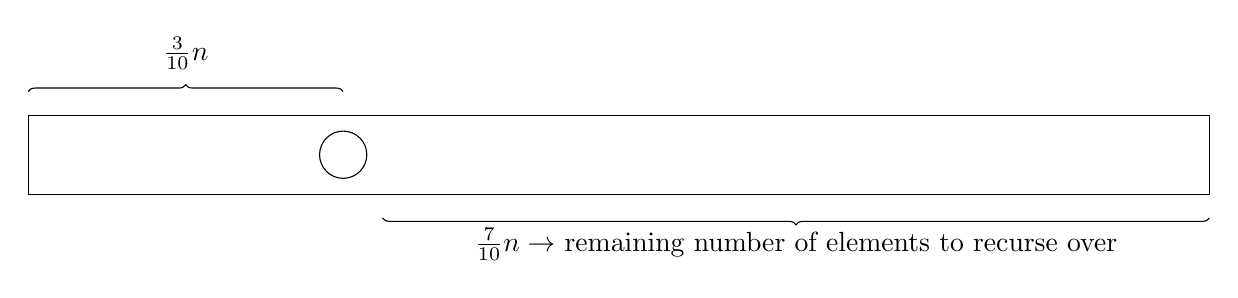
\begin{tikzpicture}

    \draw (0,0) rectangle (15,1);
    \draw[decorate, decoration={brace}, yshift=2ex]  (0,1) -- node[above=1ex] {$\frac{3}{10}n$}  (4,1);
    \draw[decorate, decoration={brace}, yshift=-2ex]  (15,0) -- node[below=0ex] {$\frac{7}{10}n \rightarrow$ remaining number of elements to recurse over}  (4.5,0);
    \draw (4,0.5) circle (0.3cm);

\end{tikzpicture}

    \begin{align*}
        T(n) &\le 2n + T(\frac{n}{5})+T(\frac{7}{10}n)+ n - 1  \\
        &= T(\frac{n}{5}) + T(\frac{7}{10}n) + 3n -1 \;\;\text{Constructive induction, guess } T(n) \le an \\
        &\le a\frac{n}{5} + an\frac{7}{10} + 3n -1 \\
        &= \left( \frac{9}{10}+3 \right)n -1 \\
        &\text{need } an \implies \;\;need\;\; \frac{9}{10}a + 3 \le a \therefore a \ge 30 \\
        \therefore T(n) &\le 30n \\
    \end{align*}

    Median is doable in linear time, but 30 is a very large coefficient.
    Compare it to quick sort at $n\lg{n}$,n must be $\sim 2^{30}$ for our
    linear median selection to be better.

\subsection{Theory}
    Say the upper bound, as some researchers claim to have found, that the upper bound on median selection is 3n.

    \begin{alignat*}{3}
        2n &< T(n) &< n 3n \\
        (2+\varepsilon)n && (3-\delta)n \\
        & T(n) \approx \frac{5}{2}n \\
    \end{alignat*}


   % ████████                           ██            ██      ██                         ██   ██   ██
  % ██░░░░░░██                  ██████ ░██           ████    ░██  █████                 ░░   ░██  ░██
 % ██      ░░  ██████  ██████  ░██░░░██░██          ██░░██   ░██ ██░░░██  ██████  ██████ ██ ██████░██      ██████████   ██████
% ░██         ░░██░░█ ░░░░░░██ ░██  ░██░██████     ██  ░░██  ░██░██  ░██ ██░░░░██░░██░░█░██░░░██░ ░██████ ░░██░░██░░██ ██░░░░
% ░██    █████ ░██ ░   ███████ ░██████ ░██░░░██   ██████████ ░██░░██████░██   ░██ ░██ ░ ░██  ░██  ░██░░░██ ░██ ░██ ░██░░█████
% ░░██  ░░░░██ ░██    ██░░░░██ ░██░░░  ░██  ░██  ░██░░░░░░██ ░██ ░░░░░██░██   ░██ ░██   ░██  ░██  ░██  ░██ ░██ ░██ ░██ ░░░░░██
 % ░░████████ ░███   ░░████████░██     ░██  ░██  ░██     ░██ ███  █████ ░░██████ ░███   ░██  ░░██ ░██  ░██ ███ ░██ ░██ ██████
  % ░░░░░░░░  ░░░     ░░░░░░░░ ░░      ░░   ░░   ░░      ░░ ░░░  ░░░░░   ░░░░░░  ░░░    ░░    ░░  ░░   ░░ ░░░  ░░  ░░ ░░░░░░
\section{Graph Algorithms}

Graph description. Can be represented as an adjacency list or adjacency matrix.

Undirected graph adjacency list representation is a bit awkward because it double counts
shared edges. Altering an edge on one vertex requires altering the edge on its
partner too. Requiring that you traverse both lists. One awkward way to
alleviate this is to keep extra pointers between the list elements in shared
edges.

\subsection{Memory Usage}

Matrix, where n = number of vertices, Memory usage = $\Theta(n^2)$

List, where m = number of edges, Memory usage = $\Theta(m+n)$

How big can m be? M can be as large as $n^2$, but will probably be smaller.

You could also use a bit matrix of size $\frac{n^2}{\text{word size}}$.

\subsection{Edge Lookup}
List: $\Theta(n)$
Matrix: $\Theta(1)$

\subsection{List all Edges}

List, Go down each index, then traverse each list. Amortized analysis is to
visit n elements. $\Theta(m+n)$.

Matrix, Go across each row, looking at all the 0s, even when you don't care
about them. $\Theta(n^2)$.

\subsection{Take aways}

Typically we want to use the Adjacency list representation, because it's linear
for in the average case.

\subsection{Changing the number of nodes }

\subsubsection{Adding Nodes}
Add dummy values that you can fill later to the next power of 2. If you have 11
nodes build a matrix with 16 columns and just read the first 11, when a new
node is added just use the dummy space, when you reach 17 you need to copy the
old matrix into the new one of size 32.

\subsubsection{Removing Nodes}

Shrink the array in a way similar to adding a node.

\subsection{Depth First Search}

\begin{algorithm}
    Mark v at visited\;
    for all v such that (u,v) is an edge and v has not been visited \;
    DFS {v}\;
\end{algorithm}

Adjacency Matrix: $O(n^2)$

Adjacency List: $O(n+m)$

\subsubsection{Applications}
    Identify Connected Components.

\subsection{Breadth First Search}

    While depth first search uses a recursive call, or a stack (which are
    naturally similar in modern machines) BFS uses a queue, which while similar
    in order analysis for most things is not naturally represented in a stack
    based machine.

    Does have some nice applications, like shortest distance algorithms.

\subsection{Identifying Connected Components}

    A graph is connected if there is a path from every vertex to every other vertex in the graph.

    A connected component is a connected subgraph, or a connection of such components.

\begin{algorithm}[H]
    \SetKwProg{Fn}{Function}{is}{end}%
    \SetKwFunction{Component}{Component}%
    \SetKwFunction{Compvisit}{Compvisit}%
    \Fn{\Component{G}}{%
        \For{all $x\in V[G]$}{%
            $visited[x] \gets False$\;
            $t\gets 0$\;
        }
        \For{all $x \in V[G]$}{%
            \If{not visited[x]}{%
                $t\gets t+1$\;
                \Compvisit[x];
            }
        }
    }

    \Fn{\Compvisit{x}}{%
        $visited[x] \gets True$\;
        $CompNum[x] \gets t$\;
        \For{all $y \in adj[x]$}{%
            \If{not visited[y]}{%
                Compvisit[y]\;
            }
        }
    }
    \caption{Connected Component}
\end{algorithm}

Adjacency Matrix: $O(n^2)$

Adjacency List: $O(n+m)$

\subsection{Bridges of K{\"o}ningsberg}

\begin{thrm}[Eulerian Cycle 1736]
    An undirected, (connected) graph $G=(v,e)$ has an Eulerian Cycle if and only if every vertex is connected and every vertex has an even degree (number of incoming and outgoing edges, with loops counted twice).
\end{thrm}

%
%
%Trees
%
%

\section{Trees}
Created by S. Jaladanki
\subsection{Definitions}

\defn[Tree]{An undirected and connected acyclic graph.}

\begin{itemize}
    \item If an edge is added between two vertices in a tree, a cycle is created
    \item If any edge is removed from this cycle, we recreate a tree
\end{itemize}

Source: \url{https://en.wikipedia.org/wiki/Minimum_spanning_tree}

\defn[Spanning Tree]{A subset of edges that form a tree and contains every vertex in the graph. It does not have cycles.}

\defn[Minimum Spanning Tree (MST)]{A spanning tree that has the lowest possible sum of edge weights}

\begin{itemize}
   \item  $m = n - 1$ There are m edges in a spanning tree in a graph with n vertices \begin{itemize}
     \item  For example, a graph with 2 vertices will have a spanning tree consisting of one edge which connects the two vertices
   \end{itemize}
 \end{itemize}

\subsection{Minimum Spanning Tree Algorithms}

There are different approaches to form the Minimum Spanning Tree of a graph, and two important algorithms are Kruskal's Algorithm and Prim's Algorithm.

\subsubsection{Kruskal's Algorithm}

In this algorithm, we go through the graph edges one at a time, from smallest edge weight to largest edge weight, and add it to a Minimum Spanning Tree (MST) as long as a cycle is not created. If the edge to add would create a cycle in the MST, it is not added and the next edge is examined. We can stop when we have n-1 edges in the MST. 

\begin{algorithm}
    Sort edges by weight so that $\lvert e_1\rvert\ \leq \lvert e_2\rvert\ \leq \lvert e_m\rvert\ $\;
    {\tcp{Assign empty tree}}
    $T \gets 0$\;
    {\tcp{m is the edges in a graph}}
    \For{$i=1$ \KwTo $m $}{%
        Put edge $i$ into $T$ if cycle is not made\;
    }
    \caption{Kruskal's Algorithm}
\end{algorithm}

\subsubsection{Prim's Algorithm}

In this algorithm, we can start at any vertex and grow the Minimum Spanning Tree (MST). We take the cheapest (smallest) edge coming off the growing tree that leads to a new vertex and add it to the MST. This process is repeated until a MST is made. 

\begin{algorithm}[H]
    \For{all $x \in V[G]$}{\tcp{Distances to all vertices initialized to $\infty$}
        $D[x] \gets \infty$\;
        {\tcp{Predecessors ($\Pi$) to all vertices initialized to NIL}}
        $\Pi[x] \gets NIL$\;
    }
    $Q \gets V[G]$ \tcp{Q will hold the vertices which haven't been checked off yet or "outside" vertices}
    {\tcp{Distance to start vertex (a) assigned 0 so it is first vertex popped from Q}}
    $D[a] \gets 0$\;
    \While{$Q \neq \emptyset$}{
        $x \gets $Pop-minimum[Q]\;
        \For{all y adjacent to x in Q}{
            \If{$y \in Q$ and $W[x,y] < D[y]$}{\tcp{W[x,y] is the weight of edge x,y}
                {\tcp{Distance and predecessor to new vertex updated}}
                $D[y] \gets W[x,y]$\;
                $\Pi[y] \gets x$\;
            }
        }
    \caption{Prim's Algorithm}
    }
    
\end{algorithm}
\BlankLine

This algorithm is nearly identical to Dijkstra's Algorithm. One important difference between these two is that Prim's adds the vertex closest to the current tree and Dijkstra's adds the vertex closest to the source vertex. 
\newline
\newline
The implementation details are similar to Dijkstra's Algorithm.

\subsubsection{Proof for Kruskal's and Prim's Algorithms}

The proof for Kruskal's and Prim's Algorithms, which are greedy algorithms, is a proof by contradiction. Let's imagine that we have a partially formed MST and that this MST has been made by adding cheapest edges to the tree. On the other side of an imaginary boundary line, there are the remaining vertices which need to be added to the MST. 
\newline
\newline
Statement: The cheapest edge to cross the boundary is in the MST.
\newline
Let's say we just added the cheapest edge (1) to cross the boundary to the MST. If this edge (1) were then removed and then replaced with another edge (2) that also crosses the boundary, then we have a contradiction because the new edge (2) is not the cheapest edge to cross the boundary because the old edge (1) was already the cheapest. Therefore, we would no longer have a MST with the new edge (2). 


 % ███████              ██   ██            ██      ██                         ██   ██   ██
% ░██░░░░██            ░██  ░██           ████    ░██  █████                 ░░   ░██  ░██
% ░██   ░██  ██████   ██████░██          ██░░██   ░██ ██░░░██  ██████  ██████ ██ ██████░██      ██████████   ██████
% ░███████  ░░░░░░██ ░░░██░ ░██████     ██  ░░██  ░██░██  ░██ ██░░░░██░░██░░█░██░░░██░ ░██████ ░░██░░██░░██ ██░░░░
% ░██░░░░    ███████   ░██  ░██░░░██   ██████████ ░██░░██████░██   ░██ ░██ ░ ░██  ░██  ░██░░░██ ░██ ░██ ░██░░█████
% ░██       ██░░░░██   ░██  ░██  ░██  ░██░░░░░░██ ░██ ░░░░░██░██   ░██ ░██   ░██  ░██  ░██  ░██ ░██ ░██ ░██ ░░░░░██
% ░██      ░░████████  ░░██ ░██  ░██  ░██     ░██ ███  █████ ░░██████ ░███   ░██  ░░██ ░██  ░██ ███ ░██ ░██ ██████
% ░░        ░░░░░░░░    ░░  ░░   ░░   ░░      ░░ ░░░  ░░░░░   ░░░░░░  ░░░    ░░    ░░  ░░   ░░ ░░░  ░░  ░░ ░░░░░░
\section{Shortest Path Algorithms}
\textbf{Types}
\begin{itemize}
    \item Single source, Single sink.
        \begin{itemize}
        \item Ex. What is the best route from site A to site B? 
        \end{itemize}
    \item All Pairs.
        \begin{itemize}
        \item Ex. What is the shortest route between every pair of cities? 
        \end{itemize}
    \item Single source.
        \begin{itemize}
        \item Ex. What is the shortest distance from A to other locations? 
        \end{itemize}
\end{itemize}

It's very hard to solve the Single source, single sink problem without also
solving the single source problem for every node along the way. Same is true
for All pairs.

\subsection{Dijkstra's Algorithm}

\begin{algorithm}[H]
    \For{all $x \in V[G]$}{\tcp{$\Theta(n)$}
        $D[x] \gets \infty$\;
        $\Pi[x] \gets NIL$\;
    }
    $Q \gets V[G]$ \tcp{Q will hold the vertices which haven't been checked off yet}
    $D[a] \gets 0$\;
    \While{$Q \neq \emptyset$}{\tcp{$\Theta(n)$}
        $x \gets $Pop-minimum[Q]\;
        \For{all y adjacent to x in Q}{\tcp{Depends on implementation. Can be adjacency matrix, checkable in $\Theta(n)$}
            \If{$D[x] + W[x,y] < D[y]$}{\tcp{W[x,y] is the weight of edge x,y}
                $D[y] \gets D[x] + W[x,y]$\;
                $\Pi[y] \gets x$\;
            }
        }
    }
\end{algorithm}

This bears a similarity to Breadth First Search. From the source, you reach the
vertices separated by 1 edge first, then those separated by 2 edges, then 3,
etc.  This forms an expanding shell of visited nodes with known shortest
distance.  We have connections to edges outside the shell, with known edge
weights. Since we are picking the smallest such edge, the BFS-like process
guarantees that you determine the shortest path to that vertex.

This only works when you have non-negative weight edges.

\subsubsection{Correctness Proof}

Base case: Nothing is in the circle, except the source vertex with distance 0.

Inductive Step: Remove smallest edge weight from consideration and update
connecting vertices if smaller.

Since you know the shortest path to everything in the circle, the available
path to the next shortest edge is guaranteed to be the shortest path to that
vertex.

\subsubsection{Implementation details}
Create Q as array. Let Q hold 1's for vertices that haven't been eliminated
yet, and 0's otherwise. Naive approach is to travel Q looking for 1, lookup
weight in D and track smallest value. If implemented with Adjacency Matrix, the
whole thing done in $\Theta(n^2)$.
\newline
\newline
The alternative is to use a priority queue / heap for Q, removing the smallest
value. This necessitates some extra heap functions to grab an arbitrary node in
the heap and change its weight. That lets you pop from the heap in logarithmic
time. There's an additional requirement to visit $|adj(x)|$ additional vertices,
and update them with our heap manipulation function to update weight, which is
an additional $\Theta(\lg n)$. Since Dijkstra's does this for every element the
running time is $\Theta(m\cdot\lg n)$.
\newline
\newline
So if your graph is dense it's better to use the Adjacency Matrix algorithm,
which is quadratic in the number of vertices. If your graph is sparse it's
better to use the $m\log n$ algorithm with a priority queue.

Of course in reality the quadratic, Adj. Matrix algorithm is usually better at
the low level because of spatial locality.


 % ████     ██ ███████          ██████                                ██           ██
% ░██░██   ░██░██░░░░██        ██░░░░██                      ██████  ░██          ░██
% ░██░░██  ░██░██   ░██       ██    ░░   ██████  ██████████ ░██░░░██ ░██  █████  ██████  █████  ███████   █████   ██████  ██████
% ░██ ░░██ ░██░███████  █████░██        ██░░░░██░░██░░██░░██░██  ░██ ░██ ██░░░██░░░██░  ██░░░██░░██░░░██ ██░░░██ ██░░░░  ██░░░░
% ░██  ░░██░██░██░░░░  ░░░░░ ░██       ░██   ░██ ░██ ░██ ░██░██████  ░██░███████  ░██  ░███████ ░██  ░██░███████░░█████ ░░█████
% ░██   ░░████░██            ░░██    ██░██   ░██ ░██ ░██ ░██░██░░░   ░██░██░░░░   ░██  ░██░░░░  ░██  ░██░██░░░░  ░░░░░██ ░░░░░██
% ░██    ░░███░██             ░░██████ ░░██████  ███ ░██ ░██░██      ███░░██████  ░░██ ░░██████ ███  ░██░░██████ ██████  ██████
% ░░      ░░░ ░░               ░░░░░░   ░░░░░░  ░░░  ░░  ░░ ░░      ░░░  ░░░░░░    ░░   ░░░░░░ ░░░   ░░  ░░░░░░ ░░░░░░  ░░░░░░
\section{NP-Completeness}

Goal is to separate problems easy to solve from those hard to solve. Loosely
speaking easy means polynomial time and hard means exponential time.

These are not perfect definitions, in spite of that fact it's still okay.

\begin{itemize}
    \item Nature is kind to us. Natural problems that are polynomial time tend to have
low degree. Not a theorem, just an empirical statement.

    \item We don't really know what a computer is. Real world computers have memory
hierarchy and variable running times, there's concurrency as well. All models
are equivalent up to polynomial time. One exception is quantum computers, but
not really proven in reality.

    \item Polynomials are closed under addition, multiplication, and composition.
% $4n^3 + 6n^2 = 4n^3 + 6n^2$
% $4n^3 \cdot 6n^2 = 24n^5$
% $4n^3 composed 6n^2 = 4{(6n^2)}^3$
\end{itemize}

\subsection{Decision Problem Theory}
Decision problems are yes/no questions.

Does a graph have an Eulerian cycle? But not What is the Eulerian Cycle.

\begin{defn}[P]
    Decision problems solvable in polynomial time.
\end{defn}

\begin{defn}[NP]
    Decision problems verifiable in polynomial time with a certificate.
\end{defn}

Problems in the class NP have the dichotomy that if the answer is yes you can
demonstrate it in polynomial time, but many of them are not able to be
disproved in polynomial time. When the answer is yes it's easy to prove, otherwise it's very hard.

Certificate is usually the solution to the problem. Example would be the coloring problem from the homework.


\begin{defn}[SAT]
Satisfiability Problem Given a Boolean formula, is there a way of setting the variables to true and
false such that the formula is true?
\end{defn}

If it is then it can be evaluated in polynomial time, the certificate is the
assignment. If it isn't satisfiable the only way to show that is to try every
possibility of assignments, which takes exponential time.

\begin{thrm}[Cook-Levin 1972]
    Satisfiability is NP-Complete.
\end{thrm}

\begin{itemize}
    \item The Cook-Levin Theorem implies that if we can solve a satisfiability problem in polynomial time, we can solve any problem in the class NP in polynomial time when the answer is "yes". 
\end{itemize}
    
\subsection{The Class of NP problems}

Is it the case that if something can be solved in polynomial time it can be verified in polynomial time?
Does $P = NP$? Or more directly, are P and NP-Complete classes distinct?
No one knows.

NP-Complete: The class of problems that are all equivalent to one another under
reduction.  Formula-SAT, circuit-SAT and coloring are all the same problem,
really. They can be reduced to one another.

Most things in real life are in the NP class. Empirical Statement: For problems
occurring in nature, Once in the class NP, it's either P or NP-Complete.
There's a theorem that says that if $P \neq NP-Complete$ then there are an
infinite class of problem between them.

\subsection{Reduction}
Having proved that a problem is NP complete, how do we prove other problems are also NP complete?

\begin{thrm}
    Circuit SAT is NP-complete.
\end{thrm}

\begin{proof}
    - Show in NP
    - Show hard for NP
    - Show that Circuit SAT is at least as hard as some other problem which we know is NP-complete.
\end{proof}

Formula SAT $\le_p$ Circuit SAT \\
Circuit SAT $\le_p$ Formula SAT \\

Converting from circuit to formula is harder than the other way. But the two
are still verifiable in the same class of running time.

\subsection{Traveling Salesman Problem}
Eulerian Cycles require that you hit every path once, while Hamiltonian Cycles
require that you hit every vertex once. This is the crux of the traveling
salesman problem. Hamiltonian Cycles are NP-Complete.

The Traveling Salesman problem is this problem of finding the shortest path that hits all the nodes in a graph.

Because the traveling salesman problem isn't a yes no question the technically
correct way of formulating it is to ask if there is a path with length less
than some target length.

This is a generalization of the Hamiltonian Cycle problem, which is NP
complete, therefore the traveling salesman problem is NP complete.

\subsubsection{Theory}
There were generalizable characteristics of the Eulerian cycle problem that
allowed Mathematicians to determine proofs around them, but the Hamiltonian
Cycle problem doesn't have any generalizable characteristics like that and it
wasn't until the advent of the NP completeness theorem that this was
understood.

\subsection{Problems between P and NP-Complete}

\begin{itemize}
    \item Factoring
    \item Discrete Logarithm
    \item Graph Isomorphism
\end{itemize}

Their exact location isn't known.

\subsection{Exam Materials}

Must prove a problem is in class NP by stating what the cert is and showing how to use the cert to verify.

No Reductions.

Show that you can use the fact of the class of the decision problem form of the
question to derive the class of the optimization problem form.  If you can
determine the yes/no condition of whether a formula is satisfiable, you can
determine the certificate for that factor in Polynomial time.
% Show that it's OK to show the decision version of a problem instead of the
% optimization version.

\subsubsection{Formula SAT}
Assume Decision version of Formula SAT is in P. We want to find the assignment.

Given Formula A variables $x_1, x_2, \ldots , x_n$

\begin{algorithm}
    \SetKwFunction{SATDEC}{SAT-decidability}%
    \If{not \SATDEC{A}}{\Return{False}}
    \For{$i=1$ \KwTo $n$}{%
        $B \gets A$\;
        Assign True to $x_i$ in A \tcp{Every time you see $x_i$ in the formula substitute with true}
            Simplify to remove True\;
        \If{not \SATDEC{A}}{%
            $A \gets B$\;
            Assign False to $x_i$ and simplify\;
        }
    }
    \Return{X}\;
\end{algorithm}

\subsubsection{Graph Coloring Problem}

Given an integer k, is a graph k-colorable?

That's the decision problem. You can use that to solve the real question of
what's the smallest number k such that a graph is k-colorable.

\begin{algorithm}[H]
    \SetKwFunction{Colorable}{Colorable}%
    $c\gets 1$\;
    \While{not \Colorable{G,c}}{%
        $c \gets c+1$\;
    }
    \For{i=1 to n}{%
        \For{d =1 to c }{%
            Set vertex i to color d\;
            \If{\Colorable{G',d}}{exit\;}
        }
    }
\end{algorithm}

    Assign arbitrary colors to the graph nodes one at a time and then ask the
    routine if the graph is still c-colorable. But assignment of colors isn't
    allowed in our routine. So we need to use a trick.

    Make a complete graph of c vertexes. Then connect our goal vertex in the
    original graph G to every vertex except the color we want. This forces the
    color determiner to require a color at that vertex.

    Size of $G^{\prime} = |G|+ c^2 +(c-1)n$

\newpage

\section{Appendices}

Created by S. Jaladanki

Here, additional information is given about concepts described in the above text.

\subsection{A. Transpositions}

A transposition involves a pair of numbers where the bigger number is above the smaller number. 
\newline
\newline
For example, let's look at an example array with the values at indices 1 to 5 listed from top to bottom. We're trying to sort this list to have lower numbers on top (or the left) and larger numbers on the bottom (the right).
\newline
\begin{align*}
    3 \\
    5 \\
    2 \\
    1 \\
    4
\end{align*}

In the above array, there are 2 transpositions involving 3, since both 1 and 2 are smaller than 3 but located farther to the bottom (or the right) than 3. There are 3 transpositions involving 5 since 2, 1, and 4 are smaller than 5 but located closer to the bottom of the array. Similarly, there is 1 transposition involving 2 (because of 1), 0 transpositions involving 1, and 0 transpositions involving 4. From the above array, there is a total of 6 transpositions. 
\newline
\newline
The number of transpositions is equal to the number of exchanges in bubble sort. For instance, in an already sorted list, there would be 0 exchanges needed since there are 0 transpositions. 

\subsection{B. Summation Properties}

Manipulating summations is an important part of the course, and examples of important properties of summations are provided.

\begin{align*}
    %\sum_{k=i}^{j}1  = j-i+1 & \text{Top index - bottom index + 1} \\
    &\sum_{k=i}^{j}1 = j-i+1 & \text{Upper limit - lower limit + 1} \\
    &\sum_{i=1}^{n}i= \frac{n(n+1)}{2} & \text{Gauss' sum formula, notice that lower limit is 1} \\
    &\sum_{i=2}^{n}(i-1) 
    =\sum_{i=1}^{n-1}(i-1)+1 = \sum_{i=1}^{n-1}i & \text{Subtract 1 from both limits and add 1 to formula}\\
    &\sum_{i=2}^{n}i 
    = (\sum_{i=1}^{n}i)-1 & \text{Since added 1 to summation, subtract 1 outside of it}\\
    &\sum_{i=1}^{n-1} 2
    = 2\sum_{i=1}^{n-1}1 & \text{Can pull out coefficients if not related to index (which is i here)}\\
    &\frac{1}{2}\sum_{i=1}^{n}(i^2+i) 
    =\frac{1}{2}\sum_{i=1}^{n}i^2 + \frac{1}{2}\sum_{i=1}^{n}i & \text{Can treat each term in parantheses as separate summation}\\
    &\sum_{i=2}^{n} \sum_{j=1}^{i}\frac{1}{i}(i-j+1) 
    =\sum_{i=2}^{n}\frac{1}{i}\sum_{j=1}^{i}(i-j+1) & \text{Can pull out $\frac{1}{i}$ from inner summation because j is index}\\
    &\sum_{i=0}^{lgn-1}2^i  
    =\frac{1-2^{(lgn-1)+1}}{1-2} = \frac{1-2^{lgn}}{-1} = -1 + n^{lg2} = n-1 & \text{Use of geometric series formula}\\
\end{align*}


Following is an example of the Change of Variable Method.

\begin{align*}
    &\sum_{i=1}^{n}(n-i+1) \\
    & \text{Writing out summation terms with substitution gives}\\
    &=\underbrace{(n-1+1)}_{n} + \underbrace{(n-2+1)}_{n-1} + \underbrace{(n-3+1)}_{n-2} + ... + 
    \underbrace{(n-(n-2)+1)}_{3} + \underbrace{(n-(n-1)+1)}_{2} + \underbrace{(n-n+1)}_{1} \\
    & \text{Based on the pattern and range of the terms (1,2,3...n-2,n-1,n) we can rewrite the summation as}\\
    &=\sum_{i=1}^{n}(i) = \frac{n(n+1)}{2} \\
\end{align*}


 % ████████ ████     ██ ███████
% ░██░░░░░ ░██░██   ░██░██░░░░██
% ░██      ░██░░██  ░██░██    ░██
% ░███████ ░██ ░░██ ░██░██    ░██
% ░██░░░░  ░██  ░░██░██░██    ░██
% ░██      ░██   ░░████░██    ██
% ░████████░██    ░░███░███████
% ░░░░░░░░ ░░      ░░░ ░░░░░░░

\end{document}